\documentclass[12pt,a4paper,oneside,english]{UPBThesis}
\setcounter{secnumdepth}{3}
\setcounter{tocdepth}{3}
\usepackage{graphicx}
\usepackage[
  bookmarksnumbered,
  bookmarks,
  bookmarksopen=true,
  pdftitle={Dissertation},
  linktocpage,
  dvips]{hyperref}
\usepackage{amsmath}
\usepackage{amssymb}
\usepackage{inputenc}
\usepackage[T1]{fontenc}
\usepackage{algpseudocode}
\usepackage{algorithm}
\usepackage{tabularx}
\usepackage{array}
\usepackage{subfigure}
\usepackage{multirow}
\usepackage{wrapfig}
\usepackage{listings}
\usepackage{tikz}
\usetikzlibrary{arrows,decorations.pathmorphing,backgrounds,positioning,fit,petri}

\floatstyle{boxed}
\restylefloat{figure}
\algrenewcommand\algorithmicrequire{\textbf{input}}
\algrenewcommand\algorithmicensure{\textbf{output}}

\newcommand{\hctimes}[2]{{#1}\!\times\!{#2}}
\newcommand{\hcrange}[2]{\overline{{#1}\colon\!\!{#2}}}
\newcommand{\hcsignalspace}{\mathbb{R}^d}
\newcommand{\hcweightspace}{\mathbb{R}^w}
\newcommand{\hcdictspace}{\mathbb{R}^{\hctimes{w}{d}}}

\singlespacing

\begin{document}

\author{Horia-Mihai COMAN}

\title{Deep Learning and Applications to Computer Vision}

\facultatea{Faculty of Electronics, Telecommunications and Information Technology}
\tiplucrare{Dissertation}
\domeniu{Applied Electronics and Information Engineering}
\catedra{Applied Electronics}
\campus{Leu}
\program{Advanced Curriculum Master Program in Imaging, Bioinformatics and Complex Systems (ITEMS)}
\titlulobtinut{Master of Science}
\director{Prof. Dr. Ing. Erhardt BARTH\\Prof. Dr. Rer. Nat. Thomas MARTINETZ\\As. Dr. Ing. \c{S}erban OPRI\c{S}ESCU}
\submissionmonth{September}
\submissionyear{2012}
\copyrightpage
\figurespage
\tablespage
\acknowledgements{The author would like to thank, for supporting this work, The German Academic Exchange Service Programme ``Ostpartnerschaften'', the University of L\"{u}beck,  and The Sectoral Operational Programme Human Resources Development 2007-2013 of the Romanian Ministry of Labour, Family and Social Protection through the Financial Agreement POSDRU/86/1.2/S/61756.}

\beforepreface


\abbreviations {
  ANN = Artificial Neural Network\\
  CNN = Convolutional Neural Network\\
  MLP = Multilayer Perceptron\\
  RBM = Restricted Boltzmann Machine\\
  LASSO = Least Absolute Shrinkage and Selection Operator\\
  MP = Matching Pursuit\\
  OMP = Orthogonal Matching Pursuit\\
  OOMP = Optimized Orhtogonal Matching Pursuit\\
  OLS = Orthogonal Least Squares\\
  PCA = Principal Component Analysis\\
  ZCA = Zero Component Analysis\\
  SVM = Support Vector Machine\\
  OLS = Ordinary Least Squares\\
}
%\preface{}
\afterpreface

\unnumberedsection{Introduction}

This thesis will study the application of new principles in Machine Learning, known under the umbrella term of Deep Learning, to the task of image recognition. The task can be formulated as a classification problem, which has been extensively studied by the Statistics and Machine Learning communities. My own contribution to this field is proposing a general architecture for classification and regression systems inspired from Deep Learning, introducing a particular form for this architecture, which, despite its simplicity, produces remarkable results on a number of benchmark problems, surpassing current state of the art results, and the usage of said architecture in a Computer Vision text detection and recognition problem.

The classification problem has received tremendous interest from the scientific community. As such, there exist efficient algorithms with a solid theoretical base such as Support Vector Machines and Classification Trees, as well as techniques for combining and boosting such methods. Each has its strengths and weaknesses, however, and when it comes to visual information processing these techniques show their limitations. Problems arise because of the very-high dimensionality of the data, because of the non-standard probability distribution which generated the data and because of non-linear dependencies between features.

There is, however, a known implementation with superb results - the human brain. For the vast majority of problems, this is the gold-standard which has yet to be beaten. It therefore seems natural to seek out ideas from studies of the brain, particularly of those regions responsible for the processing of aural and visual sensory data. While we do not have a full understanding of the brain, and not even of the first stage of visual processing, dubbed the V1 area \cite{understanding-V1,what-85percent-V1-doing}, the little we have gleamed so far has allowed us to build better systems for supervised \cite{gradient-based-learning,convolutional-networks-vision,best-practices-cnn,text-detection-character-recognition-unsupervised-feature-learning,multi-column-neural-networks,cnn-commitees-handwritten-character} and unsupervised learning \cite{high-level-features-unsupervised-feature-learning,tiny-images,reducing-dimensionality-neural-networks} of sensory data.

The form these systems take is, at its core, that of a neural network. It seem surprising that techniques which were thought surpassed by the advent of tools with a better theoretical background such as Support Vector Machines or with simpler training procedures such as Boosted Trees or Random Forests have now come back in fashion \cite{comparing-svm-cnn,mnist-website,best-architecture-object-recognition}. The truth is, of course, somewhere in between. The new neural networks are very different from the old ones. More precisely, they are truer to the real neural networks found in the brain. It has long been known that the early visual pathways had great depth, of between $10$ and $20$ layers, and the new neural networks can be, if the problem requires it, very deep, with five or six layers \cite{multi-column-neural-networks,gradient-based-learning}. For reference, the classical Multilayer Perceptron has only two. However, it is not for lack of trying that the older implementations were shallow. Rather, the training techniques known at the time did not allow bigger networks to be built. The major problem was that of ``vanishing gradients'' in the backpropagation algorithm. More precisely, as gradients were propagates from the top of the network to the bottom, they became close to zero. So much so, that lower layers would contain mostly random weights, while upper layers could not be trained properly from the mess the lower layers provided. The new techniques do not replace the backpropagation algorithm, but rather manage the inherent complexity of the problem.

The first way to do this is to restrict the allowed weights between layers. MPLs connect every neuron to to every other neuron from two consecutive layers. This means that, as with other statistical methods such as SVMs or CARTs, the input could be systematically scrambled (permuted, rotated, swapped etc.) and the methods could still produce the same results. This flies somewhat in the face of common sense. The approach taken by Convolutional Neural Networks \cite{gradient-based-learning} and variants is of maintaing the spatial or temporal structure of the inputs by linking neurons from a layer to a select group of neurons from a previous layer, usually clustered in a certain region. Thus, the number of weights is drastically reduced and the learning takes place with ``knowledge'' of the signal structure.

The second way to manage complexity is to use a different starting point for the optimization procedure. Traditionally, initial weights for the network are randomly chosen from a tightly peaked symmetric distribution around $0$. The concept of Unsupervised Pretraining replaces this with using initial weights learned from applying various unsupervised learning methods on the data, or on an unlabeled dataset similar to it. Depending on the degree of similarity, there is Semi-Supervised \cite{text-classification-semi-supervised}, Transfer \cite{text-classification-semi-supervised} or Self-Taught \cite{self-taught-learning} Learning. In any case, with such an initial setup, the learning proceeds much better, and the actual learning through back-propagation only fine-tunes the network to the particular labeled dataset.

For a general overview of the field as well as insights into why such systems work the way they do \cite{learning-deep-architectures-AI} is a good reference. Recent results have shown that, by far, the most important aspect of such a network is its structure and the particular ways in which it transforms the input. The weights might as well be random \cite{random-weights-feature-learning,beyond-simple-features}. To quantify this claim, for best results, the weights have to be pre-trained, but for architecture selection, or when insufficient data is available, random weights perform remarkably well. This thesis continues this line of research by proposing an architecture with superios performance using random weights. More generally, the task of classification is split into two parts, namely feature extraction and label decision. The feature extractor is modeled as a neural network whose task is that of mapping inputs into a high-dimensional space of such a nature that a simple classifier can work. The classifier can be a Perceptron, making the whole system a neural network, or can be a Linear SVM, a Kernelized SVM or even a Decision Tree. The major contribution is in the architecture description and the specific architecture which achieves good results.

The structure of the rest of this thesis is as follows. \textbf{Chapter \ref{chap:OverviewFeatureExtraction}} presents the high-level structure of a Deep Learning inspired feature extractor and presents the major choices available to a designer. \textbf{Chapter \ref{chap:CodingAndCodingMethods}} focuses on a major component of a feature extractor, namely the feature coding. \textbf{Chapter \ref{chap:ObtainingFeatureSet}} focuses on the another major component of a feture extractor, namely the learning of features. \textbf{Chapter \ref{chap:Experiments}} presents a number of experiments which highlight the different strengths and weaknesses of the feature coding and learning methods, as well as an example of architecture selection for two benchmark image classification problems. The strenghts of our own method and its superior results are highlighted.

We end with a description of the style conventions in use throught this thesis. Vectors are written in boldface with lower case letters - $\textbf{v}$. Addressing elment $i$ from $\textbf{v}$ is done with a subscript - $\textbf{v}_i$. Accessing a set of elements $\Lambda$ from $\textbf{v}$ is done using the set as a subscript - $\textbf{v}_\Lambda$. Matrices are written in boldface with capital letters - $\textbf{A}$. Accessing a certain column $i$ from $\textbf{A}$ is done with a superscript - $\textbf{A}^i$. Accessing a certain element $j$ in column $i$ from $\textbf{A}$ is done with both a superscript and a subscript - $\textbf{A}^i_j$. Accessing a certain set of columns $\Lambda$ from $\textbf{A}$ is done using the set as a superscript - $\textbf{A}^\Lambda$. Accessing a certain set of indices $\Lambda$ of column $i$ from $\textbf{A}$ is done using a superscript and the set as a subscript - $\textbf{A}^i_\Lambda$. Accessing a certain subset of indices $\Theta$ of a certain subset of columns $\Lambda$ from $\textbf{A}$ is done using the column set as a superscript and the element set as a subscript - $\textbf{A}^\Lambda_\Theta$. Every time a set is used for indexing, the resulting elements or columns are in increasing order of indices. [[[Talk about signal representation and linearization]]] [[[Talk about index access]]]

\chapter{Overview of Feature Extraction}
\label{chap:OverviewFeatureExtraction}

This chapter will describe the Deep Learning inspired feature extractor architecture. This kind of splitting of concerns in a classifier between feature extraction and actual decision is very old, and was one way of overcoming the inherent hardness of the problem. Humans would design certain features, that is, certain properties of an image, which are thought relevant to the application at hand. Then, these features are ``extracted'' from the the image, that is, the amount in which the image contains each feature is computed, producing the feature response vector. Finally, the actual statistical classifier is fed just the list of responses in order to obtain an predicted label. Two major tasks become apparent, namely, the design of features and the process of computing responses. \textbf{Chapter \ref{chap:CodingAndCodingMethods}} deals with the later problem while \textbf{Chapter \ref{chap:ObtainingFeatureSet}} deals with the former.

In our framework, a feature is a small image patch - a filter - of some sort. A feature set consists of $w$ normalized square images of size $d = \hctimes{p}{p}$ with $p < \min(m,n)$. We denote it by $\textbf{C} = \left[ \textbf{C}^1 \left|\right. \textbf{C}^2 \left|\right. \dots \left|\right. \textbf{C}^w \right] \in \mathbb{R}^{\hctimes{d}{w}}$ with $\|\mathbf{C}^i\| = 1$ for all $i \in \hcrange{1}{w}$. For now we consider the feature set as given. Speaking broadly, though, feature sets can be generated randomly \cite{random-weights-feature-learning,beyond-simple-features}, or taken to be a well-known set, such as DCT bases or Gabor Wavelet bases \cite{simple-method-sparse-coding}, or, even learned from a sample of patches extracted from the training set of the classification system \cite{emergence-sparse-coding,sparse-coding-strategy-V1,tiny-images}. More details about feature set construction will be given in \textbf{Chapter \ref{chap:ObtainingFeatureSet}}.

A feature extractor is composed of a number of $L$ recoding modules, linked in a serial manner. Each one has an associated set of features $\textbf{C}_l$ with $l \in \hcrange{1}{L}$. The input image is propagated through these modules and transformed by them. The first such module starts with the image $\textbf{I}$ and produces a set of images $\{\textbf{I}_i^1\}_{i=1}^{l_1}$. The next module accepts as input $\{\textbf{I}_i^1\}_{i=1}^{l_1}$ and produces $\{\textbf{I}_i^2\}_{i=1}^{l_2}$. The last module outputs $\{\textbf{I}_i^L\}_{i=1}^{l_L}$, which is linearized to produce the feature vector $\mathbf{F}$. The stacking of these module produces a deep forward path for the input image. As we will see, this transformation can be described as a neural network with many layers. \textbf{Figure \ref{fig:OverviewExHighLevelExtractor}} presents this high level view of the feature extractor.

\begin{figure}
\centering
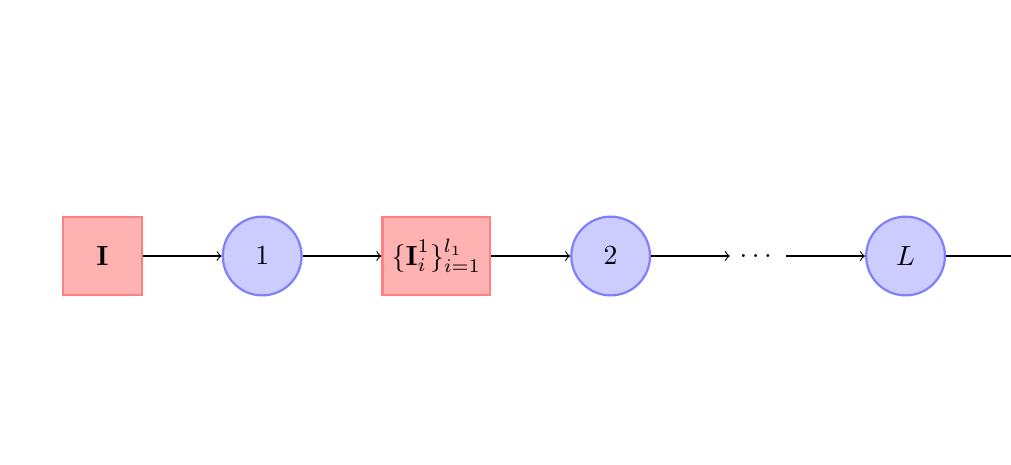
\begin{tikzpicture}
  [data/.style={rectangle,draw=red!50,thick,fill=red!30,minimum size=10mm},
   recoder/.style={circle,draw=blue!50,thick,fill=blue!20,minimum size=10mm}]
  \useasboundingbox (0,0) rectangle (\textwidth,5.2);
  \node[data] (input) at (0.95,2.3) {$\textbf{I}$};
  \node[recoder] (recoder1) [right=of input] {$1$};
  \node[data] (o_recoder1) [right=of recoder1] {$\{\textbf{I}_i^1\}_{i=1}^{l_1}$};
  \node[recoder] (recoder2) [right=of o_recoder1] {$2$};
  \node (dotsdots) [right=of recoder2] {$\dots$};
  \node[recoder] (recoderL) [right=of dotsdots] {$L$};
  \node[data] (o_recoderL) [right=of recoderL] {$\{\textbf{I}_i^L\}_{i=1}^{l_L}$};
  \node[data] (output) [right=of o_recoderL] {$\textbf{F}$};
  \draw [->] (input.east) -- (recoder1.west);
  \draw [->] (recoder1.east) -- (o_recoder1.west);
  \draw [->] (o_recoder1.east) -- (recoder2.west);
  \draw [->] (recoder2.east) -- (dotsdots.west);
  \draw [->] (dotsdots.east) -- (recoderL.west);
  \draw [->] (recoderL.east) -- (o_recoderL.west);
  \draw [->] (o_recoderL.east) -- (output.west);
\end{tikzpicture}
\caption{High level view of the feature extractor. Red nodes correspond to the different forms the input image $\textbf{I}$ passes through before the feature response $\textbf{F}$ are obtained. Blue nodes represent the different recoder modules.}
\label{fig:OverviewExHighLevelExtractor}
\end{figure}

A recoder consists of several standard steps, called \emph{coding}, \emph{nonlinear}, \emph{polarity split} and \emph{reduce}. Suppose we are working with recoder $l \in \hcrange{1}{L}$. For the sake of simpler notation, we will ommit the subscript for the parameters, stage inputs and stage outputs that will follow. 

The coding step is the only step that works directly with the input images and the feature set $\textbf{C}$. It produces a set of $w$ images $\{\textbf{I}_i^c\}_{i=1}^{w}$ of the same size as the ones in the input set. In the simplest case, where $l=1$ and the input image is actually $\textbf{I}$, each pixel $(\alpha,\beta)$ of image $q \in \hcrange{1}{w}$ represents the response of the patch of size $\hctimes{p}{p}$ centered around position $(\alpha,\beta)$ from $\textbf{I}$, to feature $\textbf{C}^q$. When $l > 1$, each pixel $(\alpha,\beta)$ of image $q \in \hcrange{1}{w}$ represents the combined response of patches of size $\hctimes{p}{p}$ centered around position $(\alpha,\beta)$ from a subset of the input images, to feature $\textbf{C}^q$. How the subsets are selected and how the patches are combined is up to the application, but usually stride patterns and patch means as seen in \cite{gradient-based-learning} are used. In the simplest case, ${\textbf{I}_q^c}(\alpha,\beta)$ depends only on the input patches and $\textbf{C}^q$. More generally, the dependence could be on the whole of $\textbf{C}$. Notice however, that no other dependencies on the input images exist. Therefore, all the input image information necessary for coding comes from the patches selected. The parameters that describe the coding step are the size of the patch $p$, the number of features $w$, the feature set $\textbf{C}$ and the coding method employed $\mathcal{C}_{\textbf{C}}$. More details about coding methods will be given in \textbf{Chapter \ref{chap:CodingAndCodingMethods}}.

The nonlinear step follows the coding step. It accepts as input the set of $w$ images produced by the coding step and outputs another set of $w$ images $\{\textbf{I}_i^n\}_{i=1}^w$ of the same size as the ones in the input set. The simplest kind of nonlinearity is using none at all. Using this \emph{Linear} nonlinearity just copies the input to this step to the output. The classical nonlinearity is the logistic one. Using this \emph{Logistic} nonlinearity, each pixel from each input image is passed independently through the sigmoid function $1 / (1 + e^{-x}) - 0.5$. Notice that this function is odd, and will nonlinearly map inputs of the same magnitude but different signs to outputs of the same magnitude and corresponding signs. \textbf{Figure \ref{fig:OverviewExNonlinearities}\subref{fig:OverviewExLogistic}} shows the form this function takes for inputs in $[-10,10]$.

One of our contributions deals with this stage. We introduce a nonlinearity based on the relative ranking between the responses to the different features. Using this \emph{Global} nonlinearity, each pixel from each output image $\textbf{I}_i^n(\alpha,\beta)$ depends on the order of $\textbf{I}_i^c(\alpha,\beta)$ in the set $Q(\alpha,\beta) = \{\textbf{I}_j^c(\alpha,\beta)\}_{j=1}^w$ of responses for position $(\alpha,\beta)$, through an exponentially decaying function of the form seen in $\textbf{Figure \ref{fig:OverviewExNonlinearities}\subref{fig:OverviewExExponentialDecay}}$. Simply put, the response for the feature with highest magnitude is mapped to $1$, the response for the feature with second highest magnitude is mapped to $0.5$ etc. The actual mapping might differ, depending on the decay function setup, but the spirit is the same. Therefore, for this type of nonlinearity, responses do not pass independently through the stage. Rather, pixels from all input images at a certain positions $(\alpha,\beta)$ are considered together when computing the output. It is a radical departure from the previous models of nonlinearity, and, one reason for the methods effectiveness, as will be shown in \textbf{Chapter \ref{chap:Experiments}}.

\begin{figure}
\centering
\subfigure[Logistic function.]{
  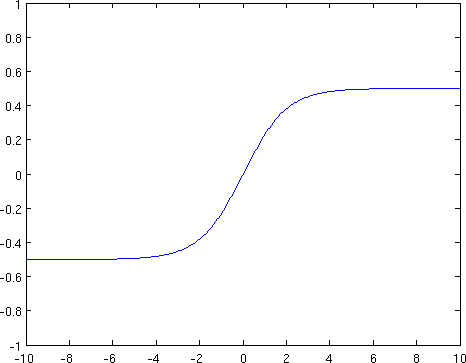
\includegraphics[width=0.40\textwidth]{thesis_data/overviewex/logistic.png}
  \label{fig:OverviewExLogistic}
}
\subfigure[Exponential decay function.]{
  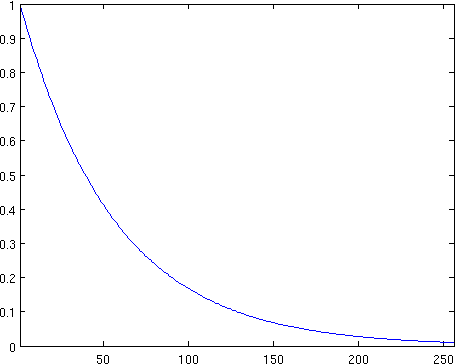
\includegraphics[width=0.40\textwidth]{thesis_data/overviewex/exponential_decay.png}
  \label{fig:OverviewExExponentialDecay}
} 
\caption{The logistic function used in the Logistic nonlinearity and the exponential decay function used as part of the Global nonlinearity. Notice that in the latter, the input is the rank of a certain response in a list of responses.}
\label{fig:OverviewExNonlinearities}
\end{figure}

The three different types of nonlinear stages are summarized in \textbf{Table \ref{table:OverviewExComputation}}. The parameter that describes the nonlinear step is the type of nonlinearity to employ $\mathcal{N}$.

\renewcommand{\arraystretch}{1.2}
\begin{table}
  \caption{The computation performed by the different stage types.}
  \label{table:OverviewExComputation}
  \newcolumntype{R}{>{\centering}X}
  \begin{tabularx}{\textwidth}{|c|c|R|}
    \hline
    Stage & Type & Computation \tabularnewline\hline\hline
    \multirow{3}{*}{Nonlinear} & Linear & $\textbf{I}_i^n(\alpha,\beta) = \textbf{I}_i^c(\alpha,\beta)$ \tabularnewline
    & Logistic & $\textbf{I}_i^n(\alpha,\beta) = {\left( 1 - \exp { \left( -\textbf{I}_i^c(\alpha,\beta) \right) } \right)}^{-1} - 0.5$ \tabularnewline
    & Global & $\textbf{I}_i^n(\alpha,\beta) = \exp \left({\frac{\mbox{rank}[Q(\alpha,\beta)](\textbf{I}_i^c(\alpha,\beta))}{w}} \right)$ \tabularnewline\hline\hline
    \multirow{5}{*}{Polarity Split} & None & $\textbf{I}_i^p(\alpha,\beta) = \textbf{I}_i^n(\alpha,\beta)$ \tabularnewline
    & \multirow{2}{*}{NoSign} & $\textbf{I}_i^p(\alpha,\beta) = \max(0,\textbf{I}_i^n(\alpha,\beta)) \mbox{~if $p \leq w$}$ \tabularnewline
    & & $\textbf{I}_i^p(\alpha,\beta) = \max(0,-\textbf{I}_i^n(\alpha,\beta)) \mbox{~if $p > w$}$ \tabularnewline
    & \multirow{2}{*}{KeepSign} & $\textbf{I}_i^p(\alpha,\beta) = \max(0,\textbf{I}_i^n(\alpha,\beta)) \mbox{~if $p \leq w$}$ \tabularnewline
    & & $\textbf{I}_i^p(\alpha,\beta) = \min(0,\textbf{I}_i^n(\alpha,\beta)) \mbox{~if $p > w$}$ \tabularnewline\hline\hline
    \multirow{5}{*}{Reduce} & Subsample & $\textbf{I}_i^r(\alpha,\beta) = \textbf{I}_i^p(\alpha,\beta)$ \tabularnewline
    & MaxNoSign & $\textbf{I}_i^r(\alpha,\beta) = \max(\left| \textbf{I}_i^p(\hcrange{\alpha}{\alpha+r},\hcrange{\beta}{\beta+r}) \right|)$ \tabularnewline
    & MaxKeepSign & $\textbf{I}_i^r(\alpha,\beta) = \max_s(\left| \textbf{I}_i^p(\hcrange{\alpha}{\alpha+r},\hcrange{\beta}{\beta+r}) \right|)$ \tabularnewline
    & SumAbs & $\textbf{I}_i^r(\alpha,\beta) = \sum_{i=0}^{r-1}{\sum_{j=0}^{r-1}{\left| \textbf{I}_i^p(\alpha+i,\beta+j) \right|}}$ \tabularnewline
    & SumSqr & $\textbf{I}_i^r(\alpha,\beta) = \sum_{i=0}^{r-1}{\sum_{j=0}^{r-1}{\textbf{I}_i^p(\alpha+i,\beta+j)^2}}$ \tabularnewline\hline
  \end{tabularx}
\end{table}

The polarity split step follows the nonlinear step. It accepts as input the set of $w$ images produced by the nonlinear step and outputs another set of $l_l=w$ or $l_l=2w$ images $\{\textbf{I}_i^p\}_{i=1}^{l_l}$ of the same size as the ones in the input set. This stage can be either on or off. If it is off, then we have the simplest case, dubbed \emph{None}. This stage has no effect and the output is simply a copy of the input. If it is on, however, the output becomes twice the size of the input, in terms of number of images. The first half contains all the coefficients which have positive sign while the second half contains all the coefficients which have negative sign. Intuitively, the input was duplicated to form the output. Then, in the first half of the image set, all negative responses were replaced by $0$ while in the second half, all positive responses were replaced by $0$. Depending on how we treat signs in the seconf half, we can have two types of polarity split, \emph{NoSign} and \emph{KeepSign}, which apply or fail to apply an absolute value on the coefficients in the second half of the output image set, respectively. The operations performed here treat, again, each pixel and each image as independent. The actual operations are nonlinear of course, but not as strict as the nonlinear stage. The three different types of polarity split stages are presented in \textbf{Table \ref{table:OverviewExComputation}}. The parameter which describes the polarity split step is the type of polarity split to employ $\mathcal{P}$.

The reduce step follows the polarity split step. It accepts as input the set of $l_l$ images produced by the polarity split step and outputs another set of $l_l$ images $\{\textbf{I}_i^r\}_{i=1}^{l_l}$ of size smaller by a factor of $r$ in both the number of rows and columns than the input set. If the number of rows and columns is not a multiple of $r$, the extra elements are discarded. It basically splits an input image into $\hctimes{r}{r}$ non-overlapping but tightly spaced patches. Coefficient $\textbf{I}_i^r(\alpha,\beta)$ is computed from all the pixels in $\textbf{I}_i^p(\hcrange{\alpha}{\alpha+r},\hcrange{\beta}{\beta+r})$. The simplest kind of reduce operation is simply to copy the top-left pixel from the input image to the output image and ignore all the others in the specific reduce region. This is called \emph{Subsample} reduce. Other approaches include the \emph{MaxNoSign} and \emph{MaxKeepSign} reduce operations, which make the output pixel be equal to the largest coefficiet, in amplitude, from the reduce region. The diffrence between the two is that in the former, no sign information is kept - only positive values are returned, while in the latter, sign information is kept. A sum of the different values can also be taken, and this is the approach used by the \emph{SumAbs} and \emph{SumSqr} reduce types, which compute a sum of absolute values or sum of squared values, respectively, from the reduce region. The five different types of reduce stages are presented in \textbf{Table \ref{table:OverviewExComputation}}. The parameters which describe the reduce stage are the tye of reduce stage $\mathcal{R}$ and the size of the reduce region $r$.

Each stage has a well-defined role and a particular performance reason for existing. The coding stage is, obviously, needed to actually extract feature responses. Without it, there is no point in continuing. What about the other stages, then? How do they affect performance? The second stage provides the necessary boost for superior performance in classification and regression problems. This is known from classical MLPs. More precisely, using artifical neurons without any kind of non-linearity, reduced the approximation powers of the MLP to that of a normal Perceptron, as the output was still just a linear combination of the input, albeit more inefficiently written. The pair of coding and nonlinear stages give the different methods their powers. Adding a polarity split stage has been observed to increase classification accuracy \cite{importance-encoding-sparse-coding-vq}. From our point of view, it is essentially free performance, since the feature vector dimensionality doubles without a corresponding increase in feature count, which would entail larger computational costs from the coding methods. Finally, the reduce stage has the role of making the recoder more resistant to small translations of the input. If a feature ``appears'' anywhere in a reduce region, the corresponding output coefficient will have a high value, regardless of exact position.

\textbf{Figure \ref{fig:OverviewExHighLevelRecoder}} shows an overview of the high-level transformations suffered by the data as it passes through a recoder. The feed-forward nature becomes apparent. However, this is not quite an ANN in the classical sense. The polarity split and reduce stages can very well be modelled as artificial neurons by an appropriate function and weight selection. The None and Logistic nonlinear stages lend themselves to such an understanding as well. However, the Global nonlinear stage as well as the kinds of coding methods we will see in \textbf{Chapter \ref{cite:CodingAndCodingMethods}} do not appear to be very amicable to such a treatement. That doens't mean the whole recoder cannot be seen as a neural network. It is - just not an MLP. Therefore, backpropagation cannot be applied unless the architecture is designed to. This has not proven a problem in practice. Good results have been obtained without fine-tuning. Moreover, we have used networks with just one recoder. The networks are still ``deep'' by MLP standards, but not as deep as could be built. This has been dictated by the properties of the datasets we benchmarked on - deeper networks were not needed. Architecture selection has become a much more important issue now. Best performance can be obtained by a rigurous search through the space of possible designs, although rules of thumb and good practices can be gleaned. Again \textbf{Chapter \ref{chap:Experiments}} provides more commentary and insights into what makes a good architecture.

\begin{figure}
\centering
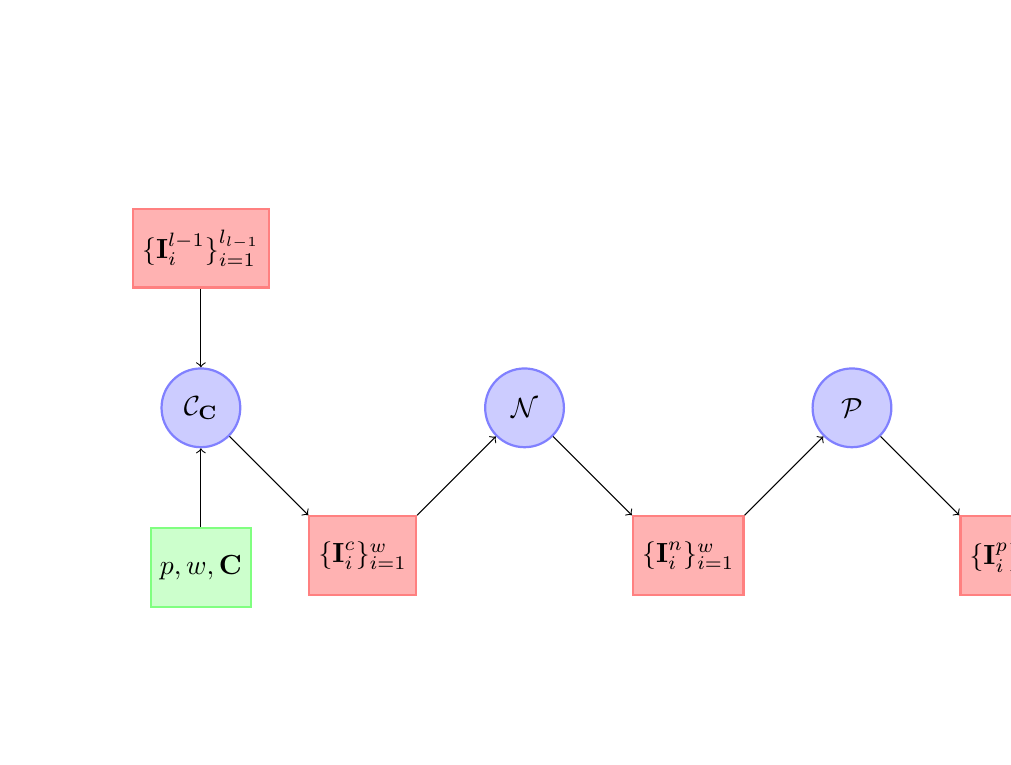
\begin{tikzpicture}
  [data/.style={rectangle,draw=red!50,thick,fill=red!30,minimum size=10mm},
   stage/.style={circle,draw=blue!50,thick,fill=blue!20,minimum size=10mm},
   param/.style={rectangle,draw=green!50,thick,fill=green!20,minimum size=10mm}]
  \useasboundingbox (0,0) rectangle (\textwidth,9);
  \node[data] (input) at (2.2,6.2) {$\{\textbf{I}_i^{l-1}\}_{i=1}^{l_{l-1}}$};
  \node[stage] (coding) [below=of input] {$\mathcal{C}_{\textbf{C}}$};
  \node[param] (p_coding) [below=of coding] {$p,w,\textbf{C}$};
  \node[data] (o_coding) [below right=of coding] {$\{\textbf{I}_i^c\}_{i=1}^{w}$};
  \node[stage] (nonlinear) [above right=of o_coding] {$\mathcal{N}$};
  \node[data] (o_nonlinear) [below right=of nonlinear] {$\{\textbf{I}_i^n\}_{i=1}^w$};
  \node[stage] (polarity_split) [above right=of o_nonlinear] {$\mathcal{P}$};
  \node[data] (o_polarity_split) [below right=of polarity_split] {$\{\textbf{I}_i^p\}_{i=1}^{l_l}$};
  \node[stage] (reduce) [above right=of o_polarity_split] {$\mathcal{R}$};
  \node[param] (p_reduce) [below=of reduce] {$r$};
  \node[data] (o_reduce) [above=of reduce] {$\{\textbf{I}_i^r\}_{i=1}^{l_l}$};
  \draw [->] (input.south) -- (coding.north);
  \draw [->] (p_coding.north) -- (coding.south);
  \draw [->] (coding.south east) -- (o_coding.north west);
  \draw [->] (o_coding.north east) -- (nonlinear.south west);
  \draw [->] (nonlinear.south east) -- (o_nonlinear.north west);
  \draw [->] (o_nonlinear.north east) -- (polarity_split.south west);
  \draw [->] (polarity_split.south east) -- (o_polarity_split.north west);
  \draw [->] (o_polarity_split.north east) -- (reduce.south west);
  \draw [->] (p_reduce.north) -- (reduce.south);
  \draw [->] (reduce.north) -- (o_reduce.south);
\end{tikzpicture}
\caption{High level view of a recoder. Red nodes correspond to the different forms the input image set passes through before the output image set is obtained. Blue nodes represent different stages. Green nodes represent parameters for blue nodes.}
\label{fig:OverviewExHighLevelRecoder}
\end{figure}

\clearpage
\newpage
\thispagestyle{empty}
\mbox{}

\chapter{Coding and Different Coding Methods}
\label{chap:CodingAndCodingMethods}

\textbf{Chapter \ref{chap:OverviewFeatureExtraction}} described the general model of a feature extractor for image processing tasks, as well as the simpler extractor we employ in this work, which uses just one recoder module. Central to this model is the coding stage which transformes the input image $\textbf{I}$ into a set of $w$ output images $\{\textbf{I}_i\}_{i=1}^w$. Image $\textbf{I}_i$ roughly corresponds to a particular feature $\textbf{C}^i$ from the feature set. Coefficient $\textbf{I}_i(\alpha,\beta)$ is the ``response'' of $\textbf{I}$ at position $(\alpha,\beta)$ to feature $\textbf{C}^i$. In general, this response can depend on the whole of $\textbf{C}$, not just on $\textbf{C}^i$.

The fundamental task of the coding stage is to obtain the set of $w$ coefficients corresponding to the patch of size $\hctimes{p}{p}$ centered at position $(\alpha,\beta)$ from $\textbf{I}$. A procedure for doing this is called a \emph{coding method}. In order to keep things simple, we will assume the inputs are $d$-dimensional signals. Thus, the $\hctimes{p}{p}$ patches previously discussed must be linearized such that $d = p^2$. We reffer to the input of a coding method as the \emph{signal} and to the output as the \emph{code}. The signal is then $\textbf{x} \in \hcsignalspace$ while the code is $\textbf{a} \in \hcweightspace$. We understand the code as a recipe for reconstructing the signal from the feature set. The most common such interpretation is that each coefficient $\textbf{a}_i$ determines in what proportion feature $\textbf{C}^i$ contributes to the reconstruction $\mathcal{R}_\textbf{C}(\textbf{a})$ of $\textbf{x}$. In other words, $\mathcal{R}_\textbf{C}$ is a linear combination of $\textbf{C}$ with coefficients provided by $\textbf{a}$. Formally, we have:

\begin{equation*}
\mathcal{R}_\textbf{C}(\textbf{a}) = \sum_{i=1}^{w}{a_i \textbf{C}^i} = \textbf{C}\textbf{a}
\end{equation*}

This section will describe several coding methods, discussing their apparent strengths and weaknesses. The final measure of power is the classification accuracy of systems built using these methods. However, there are several other quality measures which can be employed as proxies for the classificaion performance, and which are easier to work with, both theoretically and practically. A first such measure is reconstructive power, which is given by the expected squared norm of the error between the original and reconstructed signals. More precisely, given the code $\textbf{a}$, the squared Euclidean norm of the error is:

\begin{equation*}
\epsilon(\textbf{a}) = \| \textbf{x} - \textbf{C}\textbf{a} \|_2^2 = \sum_{i=1}^d {( x_i - \sum_{j=1}^w {C_j^i a_j})^2}
\end{equation*}

The associated quality measure for the coding method is $\mathbb{E} [ \epsilon(\textbf{a}) ]$. A second measure is sparseness, which is given by the expected code sparseness coefficient. The code sparseness coefficient is defined as the number of code responses greater in absolute value than a lower limit $\delta$, relative to $w$. More precisely, given the code $\textbf{a}$, its sparseness is:

\begin{equation*}
\rho(\textbf{a}) = \frac{\left| \{ a_i \left|\right. i \in \hcrange{1}{w} \wedge \left|a_i\right| > \delta \} \right|}{w}
\end{equation*}

The associated quality measure for the coding method is $\mathbb{E} [ \rho(\textbf{a}) ]$. \textbf{Chapter \ref{chap:Experiments}} will empirically compare coding methods from both a reconstruction and sparseness point of view, as well as presenting the links between the two quality measures and classification accuracy.

The simplest coding method, named \textbf{Corr}, builds $\textbf{a}$ as the inner-product between the signal and each feature. The inner-product is a useful similarity measure in the Euclidean spaces we usually work with and is directly proportional to the ``angle'' between signal and feature. Let $\textbf{a}^\star$ be the associated code for input $\textbf{x}$. This method produces it and the approximation $\textbf{C}\textbf{a}^\star$ as:

\begin{align*}
\textbf{a}^\star & = \textbf{C}^T\textbf{x} \\
\textbf{C}\textbf{a}^\star & = \textbf{C}\textbf{C}^Tx
\end{align*}

When the feature set is critically-complete and the vectors are orthonormal, then we have a perfect reconstruction because $\textbf{C}\textbf{C}^T = \mathbb{I}$ and $\textbf{C}\textbf{a}^\star = \textbf{x}$. This is the case, for example, when using DCT or certain wavelet feature sets. However, when the feature set is critically-complete and non-orthonormal or under-complete or over-complete, the reconstruction is no longer perfect. While for the first two cases, we have a ``bounded'' error between approximation and best approximation, given by $\textbf{C}^T\textbf{x} - \textbf{C}(\textbf{C}^T\textbf{C})^{-1}\textbf{C}^T\textbf{x}$, in the latter case the error norm grows as the number of features grows. The experiments will illustrate this, but it is intuitively obvious: since the reconstruction is a sum of features weighted by the response of the signal to each feature and \textbf{Corr} computes responses independently for each feature and there is no reason to thing that after a certain value of $w$, features will not be similar to the signal, the responses will have independently large values, thus the error will tend to increase as more and more terms are added.

Because of this, simply using the \textbf{Corr} coding method will yield poor results for most tasks, without extra limiting factors in the architecture. MLPs and CNNs, for example, use this method coupled with a logistic nonlinearity. The advantage of this method is that it computes each code coefficient independently. In the larger scheme of things, this means that each output pixel from the coding stage is independent from each other. Furthermore, the type of computation performed - a weighted sum - is amenable to analysis. As such, fine-tuning by back-propagation will only work when employing this method as a coding method. The next methods will lose the coefficient independence property but will gain better reconstructive and sparseness inducing properties.

In general, coding methods try to build an $\textbf{a}^\star$ that will produce the best approximation of $\textbf{x}$, usually subject to some constraints, most notably, sparseness ones. If we pose the problem as one of minimizing $\epsilon(\textbf{a})$ we stumble upon the classical least squares problem:

\begin{equation}
\textbf{a}^{\star} = \arg\min_{\textbf{a}} \frac{1}{2} \| \textbf{x} - \textbf{C}\textbf{a} \|_2^2
\end{equation}

The cost function has many nice properties which make it ammendable to analysis: it is continuos, differentiable and convex \cite{elements-statistical-learning}. The gradient with respect to $\textbf{a}$ is:

\begin{align*}
\frac{d \left( \frac{1}{2}\|\textbf{x} - \textbf{C}\textbf{a}\|_2^2 \right)}{d\textbf{a}} & = \frac{1}{2} \frac{d {\left( \textbf{x} - \textbf{C}\textbf{a} \right)}^T\left( \textbf{x} - \textbf{C}\textbf{a} \right)}{d\textbf{a}} \\
& = {\left( \textbf{x} - \textbf{C}\textbf{a} \right)}^T \frac{d \left( \textbf{x} - \textbf{C}\textbf{a} \right)}{d\textbf{a}} \\
& = - {\left( \textbf{x} - \textbf{C}\textbf{a} \right)}^T \textbf{C} \\
& = - {\left( \textbf{C}^T \left( \textbf{x} - \textbf{C}\textbf{a} \right) \right)}^T \\
& = - \textbf{C}^T \textbf{x} + \textbf{C}^T\textbf{C}\textbf{a}
\end{align*}

There are two major cases to consider: $w \leq d$ and $w > d$. The first one corresponds to $\textbf{C}$ being a tall matrix and the feature set being under-complete or critically-complete while the second one corresponds to $\textbf{C}$ being a wide matrix and the feature set being over-complete. It is the second case that interests us, as, most of the times, our feature sets will be overcomplete. We will study the first case however, as methods for the second are extensions of those for the first.

The first case admits two approaches for finding the optimum: an analytical one and an iterative one. Whichever is best depends on the situation. The analytical solution is derived from the nice properties of the cost function. More precisely, the optimum $\textbf{a}^\star$ is found as the point in $\hcweightspace$ where the gradient becomes $\textbf{0}$. We have:

\begin{align*}
- \textbf{C}^T \textbf{x} + \textbf{C}^T\textbf{C}\textbf{a}^\star & = \textbf{0} \\
\textbf{C}^T\textbf{C}\textbf{a}^\star & = \textbf{C}^T\textbf{x} \\
\textbf{a}^\star & = {\left( \textbf{C}^T\textbf{C} \right)}^{-1} \textbf{C}^T\textbf{x}
\end{align*}

To compute the reconstruction of $\textbf{x}$ we replace $\textbf{a}^\star$ in $\textbf{C}\textbf{a}^\star$ and obtain:

\begin{align*}
\textbf{C}\textbf{x} & = \textbf{C}{\left( \textbf{C}^T\textbf{C} \right)}^{-1} \textbf{C}^T\textbf{x} \\
& = \textbf{H}\textbf{x}
\end{align*}

The matrix $\textbf{H}$ is known as the hat matrix and it is a projection matrix. Since $\textbf{C}$ is tall, the matrix $\textbf{C}^T\textbf{C}$ is positive definite and it is thus invertible. A first geometric interpretatios sees $\textbf{a}^\star$ as describing the $w$-dimensional hyperplane which best approximates a function $f:\hcweightspace \rightarrow \mathbb{R}$ which is known only at $d$ points $\{(\textbf{C}(i,:),x_i)\}_{i=1}^d$. In this form, the problem is known as linear regression. A second geometric interpretation sees $\textbf{a}^\star$ as the vector in the span of the columns of $\textbf{C}$ which is closest to $\textbf{x}$. It is this latter interpretation which interests us because it tells us that the least squares solution will produce a reconstruction which is the best we can hope for with regards to $\epsilon$. The hat matrix is then the projector from $\hcsignalspace$ into the columnspace of $\textbf{C}$.

Actually computing the inverse of $\textbf{C}^T\textbf{C}$ is not recommended however, as it is both computationally expensive and numerically unstable. It turns out it is not required either. Consider the QR decomposition $\textbf{C} = \textbf{Q}\textbf{R}$, where $\textbf{Q}$ is the same size as $\textbf{C}$ and its columns form an orthonormal basis for $\hcsignalspace$ and $\textbf{R}$ is an $\hctimes{w}{w}$ matrix which is upper triangular. Computing $\textbf{a}^\star$ and $\textbf{C}\textbf{a}$ becomes, by a simple substitution:

\begin{align*}
\textbf{a}^\star & = \textbf{R}^{-1}\textbf{Q}^T\textbf{x} \\
\textbf{C}\textbf{x} & = \textbf{Q}\textbf{Q}^T\textbf{x}
\end{align*}

We have reduced the problem of finding the optimal code and reconstruction to transpose operations, matrix-vector multiplications and solving upper triangular systems of equations, all of which can be efficiently performed in $\Theta(wd)$ time. Finding $\textbf{Q}$ and $\textbf{R}$ is another story however, but $\Theta(w^2d)$ algorithms based on the Gram-Schmidt decomposition exist for this purpose. The overall time complexity is therefore $\Theta(w^2d)$. Notice also that, when $w = d$, $\textbf{Q}$ actually is an orthonormal matrix, therefore $\textbf{C}\textbf{x} = \textbf{Q}\textbf{Q}^T\textbf{x} = \textbf{x}$. We obtain perfect reconstruction, which is what we would have expected since the columnspace of $\textbf{C}$ is equal to $\hcsignalspace$.

For very large values of $d$ and $w$, performing the computations required for the analytic solution can be prohibitive. Since the minimization problem is convex, techniques from classical optimization can be used to find a suitable $\textbf{a}^\star$ without actually performing any inversion of $\textbf{C}$. This is the interative solution to the least squares problem. Most algorithms require the ability to compute the cost function as well as the gradient of this function with respect to $\textbf{a}$. Both operations can be implemented in terms of transpose operations, matrix-vector multiplications and vector additions. Actually computing them has time complexity $\Theta(wd)$ for the value of the cost function and $\Theta(wd)$ for the gradient vector at a certain $\textbf{a}$. The overall time complexity is therefore $\Theta(Twd)$, where $T$ is the number of steps required for convergence and is, hopefully, much smaller than $d$ or $w$.

In the second major case, for $w > d$, the methods we've developed so far do not produce good results. The cost function retains its nice properties, with the exception that there isn't a single unique global minima, but rather a flat region of equal lowest cost. The iterative approach will produce one of these global minima, but the analytical solution via QR decomposition will flat out not work, as it can compute at most $d$ columns of $\textbf{Q}$, leaving the other $w - d$ equal to $\textbf{0}$. The core problem is how to restrict the space of global minima, to ones which better interest us. This is an example of an ill-posed problem and it is usually solved by augmenting the cost function in some way, in order to restrict the space of possible options. What this means basically is that using only the reconstruction error as a guide for finding $\textbf{a}^\star$ is not a precise enough constraint and we need more information about the structure of a good code in order to pick the best one.

One approach which has shown good results in practice for feature learning \cite{emergence-sparse-coding,sparse-coding-strategy-V1} and classification purposes \cite{sparse-features-audio-classification,importance-encoding-sparse-coding-vq,simple-method-sparse-coding} is the restriction that the code be \emph{sparse}, that is, the code should have a small number of large magnitude coefficients and a large number of near zero coefficients. The optimal code $\textbf{a}^\star$ is then the code which best approximates $\textbf{x}$ and is sparse.

We have introduced the sparseness coefficient as a way to measure sparseness. Large values of $\rho(\textbf{a})$ indicate very dense signals, with almost no zero or close to zero values, while small values indicate sparse signals with a few large values. Another way to measure sparseness is to look at the distribution of the coefficients in a signal. \textbf{Figure \ref{fig:CodingMethodsCoeffHists}\subref{fig:CodingMethodsCoeffSparse}} shows the histogram for a sparse signal while \textbf{Figure \ref{fig:CodingMethodsCoeffHists}\subref{fig:CodingMethodsCoeffFull}} shows the histogram for a normal signal. As you can see, sparse signals have very narrow and peaker around $0$ histograms while normal signals have spread histograms.

\begin{figure}
\centering
\subfigure[Histogram for sparse signal]{
  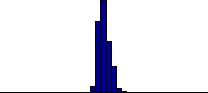
\includegraphics[width=0.40\textwidth]{thesis_data/coding_methods/coeff_sparse.png}
  \label{fig:CodingMethodsCoeffSparse}
}
\subfigure[Histogram for normal signal]{
  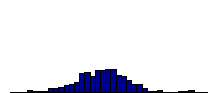
\includegraphics[width=0.40\textwidth]{thesis_data/coding_methods/coeff_full.png}
  \label{fig:CodingMethodsCoeffFull}
} 
\caption{Histograms for sparse and normal code words. There are $61$ bins spread evenly in $[-1.5,1.5]$. All horizontal axes are between $[-1.5,1.5]$ all vertical one are between $[0,250]$.}
\label{fig:CodingMethodsCoeffHists}
\end{figure}

The methods we are going to study will directly constrain either $\rho(\textbf{a})$ or the shape of the distribution in order to achieve the desired level of sparseness. The augumented optimization problem becomes:

\begin{equation*}
\textbf{a}^{\star} = \arg\min_{\textbf{a}} \frac{1}{2} \| \textbf{x} - \textbf{C}\textbf{a} \|_2^2 + \lambda \mathbb{S}(\textbf{a})
\end{equation*}

Here $\mathbb{S}$ is the sparseness constraint on the cost function while $\lambda$ is a regularization parameter which controls the tradeoff between reconstruction accuracy and sparseness.

A first method, introduced by \cite{emergence-sparse-coding} uses an $\mathbb{S}$ of the form $\sum_{i=1}^w{S(a_i / \sigma_{\textbf{a}})}$, where $\sigma$ is the standard deviation of the code word coefficients and $S$ is chosen from a set of sparsity inducing functions such as $\log(1 + x^2)$ or $-e^{-x^2}$ etc. This is one half of the SparseNet method for feature learning, adapted as a coding method. The $S$ function must be chosen such that is has small values for small absolute value inputs and large values for large absolute value inputs. The $\mathbb{S}$ constraint then will have small values when all $a_i$ are small. The only large coefficients will be forced by the reconstructing part of the problem. There is a probabilistic interpretation and derivation of SparseNet, which will be discussed in more detail in \textbf{Chapter \ref{chap:ObtainingFeatureSet}}. Suffice to say that the different forms of $S$ place a different prior or the coefficients of $\textbf{a}$, when we consider them as independently drawn from a sparse-like distribution. This method, therefore, can be considered one that tries to shape the distribution in order to achieve sparseness.

A solution to the new problem can be found only iteratively, through a modified version of the gradient based algorithm for ordinary least squares. The new formulation of the optimization problem is convex as well, though it is more difficult (from practical experience) to minimize than the simpler one. The new gradient of the cost function with respect to $\textbf{a}$ becomes:

\begin{align*}
\frac{d \left( \left( \frac{1}{2}\|\textbf{x} - \textbf{C}\textbf{a}\|_2^2 \right) + \lambda\sum_{i=1}^{w}{S(\frac{a_i}{\sigma_{\textbf{a}}})} \right)}{d\textbf{a}} & = \frac{d \left( \frac{1}{2}\|\textbf{x} - \textbf{C}\textbf{a}\|_2^2 \right)}{d\textbf{a}} + \lambda\sum_{i=1}^{w}\frac{\partial S(\frac{a_i}{\sigma_{\textbf{a}}})}{\partial a_i} \\
& = -\textbf{C}^T\textbf{x} + \textbf{C}^T\textbf{C}\textbf{a} + \frac{\lambda}{\sigma_{\textbf{a}}} \sum_{i=1}^{w} {\left( \frac{\partial S}{\partial a_i} \right) \left( \frac{a_i}{\sigma_{\textbf{a}}} \right)}
\end{align*}

Computing the cost function is $\Theta(wd)$, that is, the same, in the limit, with the ordinary least squares cost function time complexity, though, in practice, it will be a little bit slower thanks to the $\Theta(w)$ cost of computing $\mathbb{S}$, which also involves more complex operations than the addition and multiplication necessary for the approximation part. Computing the new gradient is, again, equal in the limit with the ordinary least squares gradient, that is $\Theta(wd)$, but the same remarks are valid here as for the cost function. The total time complexity will be $\Theta(Twd)$, with the mention that $T$ here might be bigger than the $T$ for the non-sparse case.

Methods that try to control $\rho(\textbf{a})$ directly all work by somehow selecting the most important features in $\textbf{C}$ and computing only the coefficients with regards to them. Examples include subset selection, forward selection and backward selection \cite{elements-statistical-learning}, which are part of a general class of feature selection algorithms, much used in Machine Learning. The canonical form for such methods is $\mathcal{L}_0$ regularized least squares, which tries to solve the following problem:

\begin{equation*}
\textbf{a}^{\star} = \arg\min_{\textbf{a}} \frac{1}{2} \| \textbf{x} - \textbf{C}\textbf{a} \|_2^2 + \lambda \| \textbf{a} \|_0
\end{equation*}

Again, $\lambda$ is the regularization parameter which controls the tradeoff between reconstruction error and sparseness, while $\|\textbf{a}\|_0$ is the $0$-norm of the code word, which is defined as $\sum_{i=1}^{w}a_i^0$ and which is equal to the number of non-null entries in $\textbf{a}$. Directly solving this problem is hard though. Luckily, it has been shown that the $\mathcal{L}_1$ regularized least squares problem, known as the \textbf{LASSO} \cite{lasso}, is a good approximation to this, and produces the good solution most of the time \cite{undetermined-minimal-L1}. There is even an efficient algorithm for solving this problem \cite{least-angle-regression}, known as Least Angle Regression. In general we can talk about the $\mathcal{L}_p$ regularized least squares problem, which solves the problem:

\begin{equation*}
\textbf{a}^{\star} = \arg\min_{\textbf{a}} \frac{1}{2} \| \textbf{x} - \textbf{C}\textbf{a} \|_2^2 + \lambda \| \textbf{a} \|_p
\end{equation*}

We will focus on a group of iterative methods for computing $\textbf{a}^\star$, known as matching pursuits, which originate in the signal processing community. The general problem they try to solve is the Lagrangian dual of the $\mathcal{L}_0$ norm least squares problem from before:

\begin{align*}
\textbf{a}^\star = \arg & \min_\textbf{a} \|\textbf{x} - \textbf{C}\textbf{a}\|_2^2 \\
& \text{~~\textbf{st}~~} \|\textbf{a}\|_0 \leq k
\end{align*}

Here $k$ is a user controlled sparseness parameter. An optimum $\textbf{a}^\star$ will have $\rho(\textbf{a}^\star) \leq k$, thereby powerfully controlling the desired sparseness. The problem is not easier to solve in this form, naturally, but it gives us a new avenue for attack, namely, we try to select the subset of $k$ features which have the minimum reconstruction error. Subset selection and forward and backward selection work on this same principle as well and are somewhat related.

The pursuit methods are greedy approximations methods. They do not solve the exact problem, but provide a good enough solution. The algorithm has a common form for all methods. In broad terms, it decomposes the original signal into smaller and smaller residual signals, which are matched with the features in $\textbf{C}$. At each step $\textbf{a}$ is filled with one new coefficient, corresponding to the feature $\omega$ which best matches the current residual. More specifically, let the initial residual $\mathcal{R}^0\textbf{x} = \textbf{x}$. At iteration $t$, let $\textbf{C}^\omega$ be the most similar feature in $\textbf{C}$, relative to $\mathcal{R}^t\textbf{x}$. The updated code and residual, $\textbf{a}^{t+1}$ and $\mathcal{R}^{t+1}\textbf{x}$, are produced by decomposing $\mathcal{R}^t\textbf{x}$ in terms of $\textbf{C}^\omega$. After $k$ iterations, $\textbf{a}^k$ is returned as the code associated to $\textbf{x}$, and $\mathcal{R}^k\textbf{x}$ is returned as a measure of the ability of the algorithm to reconstruct the signal in terms of $\textbf{C}$. The difference between the several methods consists in how they find $\textbf{C}^\omega$ and how they update $\textbf{a}^{t+1}$. The general procedure is illustrated in \textbf{Algorithm \ref{algo:GeneralPursuitMethod}}. At the end of this algorithm we obtain $\textbf{x} = \textbf{C}\textbf{a}^k + \mathcal{R}^k\textbf{x}$.

Also, the norm of the final residual $\mathcal{R}^k\textbf{x}$ tends to $0$ as $k \rightarrow +\infty$ for sensible choices of $\text{\textbf{sim}}$ and $\text{\textbf{next}}$ functions. In the limit, the equality becomes $\textbf{x} = \textbf{C}\textbf{a}^{+\infty}$, that is, perfect approximation is obtained.

\begin{algorithm}
\caption{The General Pursuit Method}
\label{algo:GeneralPursuitMethod}
\begin{algorithmic}
\Require $\textbf{C},\textbf{x},k$
\Ensure $\textbf{a}^k,\mathcal{R}^k\textbf{x}$
\State $\Lambda^0 \gets \phi$
\State $\textbf{a}^0 \gets \textbf{0}$
\State $\mathcal{R}^0\textbf{x} \gets \textbf{x}$
\For {$t = \hcrange{1}{k}$}
\State $\omega \gets \arg \max_{i \in \textbf{dom}} \text{\textbf{sim}}(\mathcal{R}^{t-1}\textbf{x},\textbf{C},\Lambda^{t-1},i)$
\State $\Lambda^t \gets \Lambda^{t-1} \cup \omega$
\State $\textbf{a}^t \gets \text{\textbf{next}}(\textbf{a}^{t-1},\mathcal{R}^{t-1}\textbf{x},\textbf{C},\Lambda^t,\omega)$
\State $\mathcal{R}^t\textbf{x} \gets \mathcal{R}^{t-1}\textbf{x} - a_\omega^t\textbf{C}^\omega$
\EndFor
\end{algorithmic}
\end{algorithm}

\renewcommand{\arraystretch}{1.5}
\begin{table}
  \caption{The different parametrization for pursuit methods}
  \label{table:PursuitParametrization}
  \begin{tabularx}{\textwidth}{|l|>{\centering}X|>{\centering}X|c|}
       \hline
        Method & $\text{\textbf{sim}}$ function & $\text{\textbf{next}}$ function & $\text{\textbf{dom}}$ domain\\ \hline \hline
        \textbf{MP} & $\left| \langle \mathcal{R}^{t-1}\textbf{x} , \textbf{C}^i \rangle \right|$ & $\textbf{a}^{t-1} + \langle \mathcal{R}^{t-1}\textbf{x} , \textbf{C}^\omega \rangle \delta_\omega$ & $\hcrange{1}{w}$ \\  \hline
        \textbf{OMP} & $\left| \langle \mathcal{R}^{t-1}\textbf{x} , \textbf{C}^i \rangle \right|$ & $\arg\min_{\textbf{a}} {\| \textbf{x} - \textbf{C}^{\Lambda^t}\textbf{a} \|_2^2}$ & $\hcrange{1}{w} \setminus \Lambda^{t-1}$ \\ \hline
        \textbf{OOMP} & $\min_{\textbf{a}} {\| \textbf{x} - \textbf{C}^{\Lambda^{t-1} \cup i}\textbf{a} \|_2^2}$ & $\arg\min_{\textbf{a}} {\| \textbf{x} - \textbf{C}^{\Lambda^t}\textbf{a} \|_2^2}$ & $\hcrange{1}{w} \setminus \Lambda^{t-1}$ \\
       \hline
    \end{tabularx}
\end{table}
\renewcommand{\arraystretch}{1.0}

The simplest pursuit method, introduced in \cite{matchingpursuit1}, is Matching Pursuit (\textbf{MP}). \textbf{Table \ref{table:PursuitParametrization}} shows what form the $\text{\textbf{sim}}$ and $\text{\textbf{next}}$ functions take in this case. An important property of this algorithm is that for every $t$, $\|\mathcal{R}^t\textbf{x}\|_2^2 \geq \|\mathcal{R}^{t+1}\textbf{x}\|_2^2$ and, furthermore, with a decay that is exponential. The two major drawbacks of this method are that the approximation at time $t$, $\textbf{C}\textbf{a}^t$, is not optimal with respect to the selection of features $\Lambda^t$; and that for the residual norm to actually reach small enough values, a $k > w$ could be necessary. However, these drawbacks are not critical for classification purposes, and, because of its simplicity and speed, we use it in our experiments. $\mathcal{R}^t\textbf{x}$ is orthogonal with respect to $\textbf{C}^\omega$, but not necesarily to every other feature in $\textbf{C}^{\Lambda^t \setminus \omega}$.

The specialization of the General Pursuit Method to Matching Pursuit can be seen in \textbf{Algorithm \ref{algo:MatchingPursuitMethodV1}}.

\begin{algorithm}
\caption{The Matching Pursuit Method (Version 1)}
\label{algo:MatchingPursuitMethodV1}
\begin{algorithmic}
\Require $\textbf{C},\textbf{x},k$
\Ensure $\textbf{a}^k,\mathcal{R}^k\textbf{x}$
\State $\Lambda^0 \gets \phi$
\State $\textbf{a}^0 \gets \textbf{0}$
\State $\mathcal{R}^0\textbf{x} \gets \textbf{x}$
\For {$t = \hcrange{1}{k}$}
\State $\omega \gets \arg \max_{i \in \hcrange{1}{w}} \left| \langle \mathcal{R}^{t-1}\textbf{x}, \textbf{C}^i \rangle \right|$
\State $\Lambda^t \gets \Lambda^{t-1} \cup \omega$
\State $\textbf{a}_\omega^t \gets \textbf{a}_\omega^{t-1} + \langle \mathcal{R}^{t-1}\textbf{x} , \textbf{C}^\omega \rangle$
\State $\mathcal{R}^t\textbf{x} \gets \mathcal{R}^{t-1}\textbf{x} - a_\omega^t\textbf{C}^\omega$
\EndFor
\end{algorithmic}
\end{algorithm}

The runtime of this variant is $T_1^{MP} = \Theta(kwd)$. This is somewhat suboptimal, as, in most cases, it will be quadratic in $d$ ($d$ and $w$ tend to have the same order of magnitude), or even cubic in $d$ for cases where $k$ has the same order of magnitude with $d$. The source of this complexity is the small optimization problem we have to solve in the inner loop. This just requires a walk through all the features and computing of a ``similarity'' of cost $\Theta(d)$. The per iteration time is therefore $\Theta(dw)$. Notice, however the following decomposition of $\mathcal{R}^t\textbf{x}$:

\begin{align*}
\mathcal{R}^t\textbf{x} & = \mathcal{R}^{t-1}\textbf{x} - a_\omega^t\textbf{C}^\omega \\
\mathcal{R}^t\textbf{x} & = \mathcal{R}^{t-1}\textbf{x} - \langle \mathcal{R}^{t-1}\textbf{x}, \mathcal{C}^\omega \rangle \textbf{C}^\omega
\end{align*}

Now, if we want to compute the inner product between $\mathcal{R}^t\textbf{x}$ and a $\textbf{C}^i$, we have:

\begin{align*}
\langle \mathcal{R}^t\textbf{x}, \textbf{C}^i \rangle & = \langle \mathcal{R}^{t-1}\textbf{x} - \langle \mathcal{R}^{t-1}\textbf{x}, \mathcal{C}^\omega \rangle \textbf{C}^\omega , \textbf{C}^i \rangle \\
& = \langle \mathcal{R}^{t-1}\textbf{x}, \textbf{C}^i \rangle - \langle \mathcal{R}^{t-1}\textbf{x}, \textbf{C}^\omega \rangle \langle \textbf{C}^\omega, \textbf{C}^i \rangle
\end{align*}

Thus, we have expressed the computation of the inner product between the current residual and a feature in terms of the inner product between the previous residual and the same feature and an ``adjustement term'', which is a product of the maximum inner product of the previous iteration and the inner product of the best previous feature and the current feature under consideration. The new algorithm can be seen in \textbf{Algorithm \ref{algo:MatchingPursuitMethodV2}}.

\begin{algorithm}
\caption{The Matching Pursuit Method (Version 2)}
\label{algo:MatchingPursuitMethodV2}
\begin{algorithmic}
\Require $\textbf{C},\textbf{x},k$
\Ensure $\textbf{a}^k,\mathcal{R}^k\textbf{x}$
\State $\textbf{a}^0 \gets \textbf{0}$
\State $\mathcal{S}^f \gets \textbf{C}^T\textbf{C}$
\State $\mathcal{S}^s \gets \textbf{C}\textbf{x}$
\For {$t = \hcrange{1}{k}$}
\State $\omega \gets \arg \max_{i \in \hcrange{1}{w}} \left| \mathcal{S}_i^s \right|$
\State $\textbf{a}_\omega^t \gets \textbf{a}_\omega^{t-1} + \mathcal{S}_\omega^s$
\State $\mathcal{S}^s \gets [ \mathcal{S}_i^s - \mathcal{S}_\omega^s \mathcal{S}_{\omega i}^f ~ \mbox{\textbf{for} $i \in \hcrange{1}{w}$} ]$
\EndFor
\end{algorithmic}
\end{algorithm}

As it is, the runtime of this algorithm is $T_2^{MP} = \Theta(w^2d + kw)$, which does not seem like much of an improvement. However, in the broad picture, many patches are coded with the same feature set. Therefore, we need to compute only once $\mathcal{S}^f$, and then use it for all patches. The average time complexity for coding $N$ patches if $\Theta(w^2d/N + kw)$ which tends to $\Theta(kw)$ for large enough $N$. Therefore, the actual time complexity is $T_2^{MP} = \Theta(kw)$, which is an order of magnitude lower than the original time $T_1^{MP}$.

An improvement to \textbf{MP} is Orthogonal Matching Pursuit (\textbf{OMP}) \cite{matchingpursuit2,orthopursuit}, which addresses the two issues discussed above. Again, \textbf{Table \ref{table:PursuitParametrization}} shows the forms the $\text{\textbf{sim}}$ and $\text{\textbf{next}}$ functions take. Also, notice that at each iteration, only the features not considered before are processed. All the properties of \textbf{MP} hold here as well. At iteration $t$ we solve a classical least squares problem with the subset of features in $\Lambda^t$. This makes sense, because the matrix will always be tall - $\left| \Lambda^t \right| \leq d$ - otherwise we produce a $0$ norm residual which effectively stops the algorithm. The algorithm is presented in \textbf{Algorithm \ref{algo:OrthogonalMatchingPursuitMethodV1}}.

\begin{algorithm}
\caption{Orthogonal Matching Pursuit (Version 1)}
\label{algo:OrthogonalMatchingPursuitMethodV1}
\begin{algorithmic}
\Require $\textbf{C},\textbf{x},k$
\Ensure $\textbf{a}^k,\mathcal{R}^k\textbf{x}$
\State $\Lambda^0 \gets \phi$
\State $\textbf{a}^0 \gets \textbf{0}$
\State $\mathcal{R}^0\textbf{x} \gets \textbf{x}$
\For {$t = \hcrange{1}{k}$}
\State $\omega \gets \arg \max_{i \in \hcrange{1}{w} \setminus \Lambda^{t-1}} \left| \langle \mathcal{R}^{t-1}\textbf{x} , \textbf{C}^i \rangle \right|$
\State $\Lambda^t \gets \Lambda^{t-1} \cup \omega$
\State $\textbf{a}^t \gets \arg\min_{\textbf{a}} {\| \textbf{x} - \textbf{C}^{\Lambda^t}\textbf{a} \|_2^2}$
\State $\mathcal{R}^t\textbf{x} \gets \mathcal{R}^{t-1}\textbf{x} - a_\omega^t\textbf{C}^\omega$
\EndFor
\end{algorithmic}
\end{algorithm}

Therefore, at iteration $t$, we chose the feature $\textbf{C}^\omega$ of maximum ``similarity'' according to the inner product measure. We add this to the current feature set $\textbf{C}^{\Lambda^t}$. In order to compute $\textbf{a}^t$ we find the point $\textbf{a}$ in the column space of $\textbf{C}^{\Lambda^t}$ closest to $\textbf{x}$ as the solution of the least squares problem. This solves the major problem of \textbf{MP}, that is, the found $\textbf{a}^k$ was not even optimal in the approximation sense to the input signal. \textbf{OMP} produces such a solution, guaranteed, and, more importantly, uses the information continuously to drive the search for new features, instead of just at the end, as a naive modification of $\textbf{MP}$ might suggest. Notice however, that, even though the solution found has minimum approximation error, it is only in respect to the subset of features selected. There is no guarantee that there isn't a better solution with regards to another subset, or a solution of the same cost but using a smaller number of features. We are not solving an $NP$-hard problem in polynomial time with this algorithm.

The major problem of the \textbf{OMP} algorithm, as it is, is the extra complexity introduced by the need to solve the least squares problem. We have $T_1^{OMP} = \Theta(kwd + kT^{LS}))$. We know that $T^{LS} = \Theta(w^2d)$ if we use the analytical solution, therefore we have $T_1^{OMP} = \Theta(kwd + kw^2d) = \Theta(kw^2d)$, which is an order of magnitude larger than the naive algorithm time complexity for \textbf{MP}. This is somewhat prohibitive. However, an approach suggested by \cite{matchingpursuit2,pursuitdifferences} combines the computation of the QR factorization with the gradual update ideas from the second version of the Matching Pursuit.

The QR decomposition can be computed using the Gram-Schmidt process. This builds $\textbf{Q}$ one column at a time and $\textbf{R}$ one column at a time. Furthermore, the building of column $i \in \hcrange{1}{t}$ depends only on columns $\hcrange{1}{i}$ from $\textbf{C}^{\Lambda^t}$ and columns $\hcrange{1}{i-1}$ from $\textbf{Q}$. Also, the matrices $\textbf{C}^{\Lambda^t}$ and $\textbf{C}^{\Lambda^{t+1}}$ are identical, except the latter has one extra column. Using our notation, this column, corresponding to position $\omega^{t+1} \in \hcrange{1}{w}$, is inserted ``between'' two other columns from $\textbf{C}^{\Lambda^t}$. However, for our purposes, the order of the columns is irrelevant. Therefore we can consider $\textbf{C}^{\Lambda^{t+1}} = \left[\textbf{C}^{\Lambda^t} \left|\right. \textbf{C}^{\omega^{t+1}} \right]$. The two matrices have the same first $t$ columns, therefore, the first $t$ columns of the associated $\textbf{Q}$ matrices of the QR decomposition will be identical. The same goes for the first $t$ rows of the $\textbf{R}$ matrices. This naturally leads us to the version of the algorithm which accumulates the $\textbf{Q}$ and $\textbf{R}$ matrices.

Another optimization follows concerns the residual $\mathcal{R}^t\textbf{x}$ after time $t$. We have:

\begin{align*}
\mathcal{R}^t\textbf{x} & = \textbf{x} - \textbf{C}^{\Lambda^t}\textbf{a}^t \\
& = \textbf{x} - \textbf{Q}\textbf{Q}^T\textbf{x}
\end{align*}

Making use of the fact that the $\textbf{Q}$ matrix used in the computation of $\mathcal{R}^{t+1}\textbf{x}$ contains just one extra column besides the one used in the computation of $\mathcal{R}^t\textbf{x}$, we have:

\begin{align*}
\textbf{Q}_t^T\textbf{x} & = [ \langle \textbf{Q}_t^1, \textbf{x} \rangle \cdots \langle \textbf{Q}_t^t, \textbf{x} \rangle ] \\
\textbf{Q}_{t+1}^T\textbf{x} & = [ \langle \textbf{Q}_{t+1}^1, \textbf{x} \rangle \cdots \langle \textbf{Q}_{t+1}^t, \textbf{x} \rangle \langle \textbf{Q}_{t+1}^{t+1}, \textbf{x} \rangle ] \\
& = [ \langle \textbf{Q}_t^1, \textbf{x} \rangle \cdots \langle \textbf{Q}_t^t, \textbf{x} \rangle \langle \textbf{Q}_{t+1}^{t+1}, \textbf{x} \rangle] \\
\end{align*}

Therefore, computing $\textbf{Q}_{t+1}^T\textbf{x}$ needs just the $\Theta(d)$ time needed for $\langle \textbf{Q}_{t+1}^{t+1}, \textbf{x} \rangle$. Then, we have that:

\begin{align*}
\textbf{Q}_t\textbf{Q}_t^T\textbf{x} & = \sum_{i=1}^t {\langle \textbf{Q}_t^i, \textbf{x} \rangle \textbf{Q}_t^i} \\
\textbf{Q}_{t+1}\textbf{Q}_{t+1}^T\textbf{x} & = \sum_{i=1}^{t+1} {\langle \textbf{Q}_{t+1}^i, \textbf{x} \rangle \textbf{Q}_{t+1}^i} \\
& = \textbf{Q}_t\textbf{Q}_t^T\textbf{x} + \langle \textbf{Q}_{t+1}^{t+1}, \textbf{x} \rangle \textbf{Q}_{t+1}^{t+1}
\end{align*}

Thus, we can come up with a new way of computing the residual:

\begin{equation*}
\mathcal{R}^t\textbf{x} \gets \mathcal{R}^{t-1}\textbf{x} - \langle \textbf{Q}_{t}^{\omega}, \textbf{x} \rangle \textbf{Q}_{t}^{\omega}
\end{equation*}

The algorithm is presented now in \textbf{Algorithm \ref{algo:OrthogonalMatchingPursuitMethodV2}}. Notice we don't need to compute $\textbf{a}^t$ at all during the inner-loop, but only at the end. Unfortunately, we don't have a fast computation for the residual with this algorithm, as we did with \textbf{MP}. This is not such a big problem though, as the running time of the algorithm would still be the same, as there are other, more complex operations going on in the inner-loop. It would have been only a practical speedup.

\begin{algorithm}
\caption{Orthogonal Matching Pursuit (Version 2)}
\label{algo:OrthogonalMatchingPursuitMethodV2}
\begin{algorithmic}
\Require $\textbf{C},\textbf{x},k$
\Ensure $\textbf{a}^k,\mathcal{R}^k\textbf{x}$
\State $\Lambda^0 \gets \phi$
\State $\textbf{a}^0 \gets \textbf{0}$
\State $\mathcal{R}^0\textbf{x} \gets \textbf{x}$
\State $\textbf{Q} \gets \textbf{0}$
\State $\textbf{R} \gets \textbf{0}$
\State $(\textbf{Q}^T\textbf{x}) \gets \textbf{0}$
\For {$t = \hcrange{1}{k}$}
\State $\omega \gets \arg \max_{i \in \hcrange{1}{w} \setminus \Lambda^{t-1}} \left| \langle \mathcal{R}^{t-1}\textbf{x} , \textbf{C}^i \rangle \right|$
\State $\Lambda^t \gets \Lambda^{t-1} \cup \omega$
\State $\textbf{R}^t \gets [ \langle \textbf{C}^\omega, \textbf{Q}^i \rangle~\mbox{\textbf{for} $i \in \hcrange{1}{d}$ \textbf{if} $i < t$ \textbf{else} $0$} ]$ \Comment{Fill column $t$ of $\textbf{R}$}
\State $\textbf{Q}^t \gets \textbf{C}^\omega - \textbf{Q}^{\hcrange{1}{t-1}}\textbf{R}^t_{\hcrange{1}{t-1}}$ \Comment{Substract projection of $\textbf{C}^\omega$ on all $\textbf{Q}^i$ from $\textbf{C}^\omega$}
\State $\textbf{Q}^t \gets \textbf{Q}^t / \| \textbf{Q}^t \|_2$ \Comment{Normalize column $t$ of $\textbf{Q}$}
\State $\textbf{R}^t_t \gets \langle \textbf{C}^\omega, \textbf{Q}^t \rangle$
\State $(\textbf{Q}^T\textbf{x})_t \gets \langle \textbf{x}, \textbf{Q}^t \rangle$
\State $\mathcal{R}^t\textbf{x} \gets \mathcal{R}^{t-1}\textbf{x} -  (\textbf{Q}^T\textbf{x})_t \textbf{Q}^t$
\EndFor
\State $\textbf{a}_{\Lambda^k}^k \gets \textbf{R}^{-1}(\textbf{Q}^T\textbf{x})$
\end{algorithmic}
\end{algorithm}

The running time of this algorithm is $T_2^{OMP} = \Theta(dk^2)$, which is much better than $T_1^{OMP}$, but an order of magnitude larger than $T_2^{MP}$. This was to be expected however, given the greater amount of work the algorithm does, as well as its more robust properties. Another nice property of \textbf{OMP} is that $\mathcal{R}^t\textbf{x}$ is orthogonal to the span of $\textbf{Q}^1,\dots,\textbf{Q}^{t-1}$.

A final pursuit method studied is Optimized Orthogonal Matching Pursuit (\textbf{OOMP}) \cite{optimizedorthopursuit,orthogonalls} also known as Orthogonal Least Squares (\textbf{OLS}). It is similar to \textbf{OMP}. The major difference is the way in which the decision for which $\textbf{C}^\omega$ to use is taken. We select the one feature which gives the smallest least squares difference between $\textbf{x}$ and its reconstruction, that is, the feature $\omega$ which will cause the residual $\mathcal{R}^t\textbf{x}$ comptuted after the inner-loop iteration, to have the smallest norm. Once this decision has been made, however, the behaviour is identical to $\textbf{OMP}$ and the same optimality and orthogonality properties hold. The algorithm is presented in \textbf{Algorithm \ref{algo:OptimizedOrthogonalMatchingPursuitMethodV1}}.

\begin{algorithm}
\caption{Optimized Orthogonal Matching Pursuit (Version 1)}
\label{algo:OptimizedOrthogonalMatchingPursuitMethodV1}
\begin{algorithmic}
\Require $\textbf{C},\textbf{x},k$
\Ensure $\textbf{a}^k,\mathcal{R}^k\textbf{x}$
\State $\Lambda^0 \gets \phi$
\State $\textbf{a}^0 \gets \textbf{0}$
\State $\mathcal{R}^0\textbf{x} \gets \textbf{x}$
\For {$t = \hcrange{1}{k}$}
\State $\omega \gets \arg \min_{i \in \hcrange{1}{w} \setminus \Lambda^{t-1}} \min_{\textbf{a}} {\| \textbf{x} - \textbf{C}^{\Lambda^{t-1} \cup i}\textbf{a} \|_2^2}$
\State $\Lambda^t \gets \Lambda^{t-1} \cup \omega$
\State $\textbf{a}^t \gets \arg\min_{\textbf{a}} {\| \textbf{x} - \textbf{C}^{\Lambda^t}\textbf{a} \|_2^2}$
\State $\mathcal{R}^t\textbf{x} \gets \mathcal{R}^{t-1}\textbf{x} - a_\omega^t\textbf{C}^\omega$
\EndFor
\end{algorithmic}
\end{algorithm}

Again, the biggest problem for this method is the prohibitive running cost. We have to solve several least squares problems for each iteration of the algorithm. The running time is $T_1^{OOMP} = \Theta(kwT^{LS})$. The ideas which led to the second version of \textbf{OMP} can be employed here as well. We again iteratively build the $\textbf{Q}$ and $\textbf{R}$ matrices. For our purposes, it is enough to notice that for computing the actual residual, only $\textbf{Q}$ is needed. Combing this with our previous knowledge, we can reformulate the optimization problem as such:

\begin{align*}
\omega & \gets \arg\min_{i \in \hcrange{1}{w} \setminus \Lambda^{t-1}} \min_\textbf{a} \| \textbf{x} - \textbf{C}^{\Lambda^{t-1} \cup i}\textbf{a} \|_2^2 \\
& \gets \arg\min_{i \in \hcrange{1}{w} \setminus \Lambda^{t-1}} \| \textbf{x} - \textbf{Q}^{\Lambda^{t-1} \cup i}{\textbf{Q}^{\Lambda^{t-1} \cup i}}^T\textbf{x} \|_2^2 \\
& \gets \arg\min_{i \in \hcrange{1}{w} \setminus \Lambda^{t-1}} \| \mathcal{R}^{t-1}\textbf{x} - \langle \textbf{Q}^i, \textbf x \rangle \textbf{Q}^i \|_2^2
\end{align*}

Therefore we have reduced the complex $\Theta(wT^{LS})$ runtime of the first inner-loop step to $\Theta(wd)$. Quite an improvement! However, as it stands now, the $\textbf{Q}^i$ must be computed at each iteration for each one of the $w - t$ remaining features. We introduce the $\tilde{\textbf{C}}$ matrix of dimension equal to $\textbf{C}$. This is set initially as:

\begin{equation*}
\tilde{\textbf{C}} = \left[ \frac{\textbf{C}^1}{\|\textbf{C}^1\|_2} \left|\right. \dots \left|\right. \frac{\textbf{C}^w}{\|\textbf{C}^w\|_2} \right]
\end{equation*}

It contains the $\textbf{Q}^i$ at the first iteration. In general, at iteration $t$, after $\omega$ is found, each column of $\tilde{\textbf{C}}$ is updated as:

\begin{align*}
\tilde{\textbf{C}}^i & \gets \tilde{\textbf{C}}^i - \langle \tilde{\textbf{C}}^i, \tilde{\textbf{C}}^\omega \rangle \tilde{\textbf{C}}^\omega \\
\tilde{\textbf{C}}^i & \gets \tilde{\textbf{C}}^i / \| \tilde{\textbf{C}}^i \|_2
\end{align*}

At the end of the $k$ iterations, $k$ columns will be zero. Furthermore, at the start of each iteration, $\tilde{\textbf{C}}$ contains the features in $\textbf{C}$, orthogonalized with respect to $\textbf{Q}^1, \dots, \textbf{Q}^{t-1}$ and normalized. \textbf{Algorithm \ref{algo:OptimizedOrthogonalMatchingPursuitV2}} shows this second form of the \textbf{OOMP} algorithm.

\begin{algorithm}
\caption{Optimized Orthogonal Matching Pursuit (Version 2)}
\label{algo:OptimizedOrthogonalMatchingPursuitV2}
\begin{algorithmic}
\Require $\textbf{C},\textbf{x},k$
\Ensure $\textbf{a}^k,\mathcal{R}^k\textbf{x}$
\State $\Lambda^0 \gets \phi$
\State $\textbf{a}^0 \gets \textbf{0}$
\State $\mathcal{R}^0\textbf{x} \gets \textbf{x}$
\State $\textbf{R} \gets \textbf{0}$
\State $(\textbf{Q}^T\textbf{x}) \gets \textbf{0}$
\State $\tilde{\textbf{C}} \gets [ \textbf{C}^i / \|\textbf{C}^i\|_2 ~ \mbox{\textbf{for} $i \in \hcrange{1}{w}$} ]$
\For {$t = \hcrange{1}{k}$}
\State $\omega \gets \arg\min_{i \in \hcrange{1}{w} \setminus \Lambda^{t-1}} \| \mathcal{R}^{t-1}\textbf{x} - \langle \textbf{x}, \tilde{\textbf{C}}^i \rangle \tilde{\textbf{C}}^i \|_2^2$  \Comment{Choose $i$ such that residual is minimized}
\State $\Lambda^t \gets \Lambda^{t-1} \cup \omega$
\State $\textbf{R}^t \gets [ \langle \textbf{C}^\omega, \textbf{Q}^i \rangle~\mbox{\textbf{for} $i \in \hcrange{1}{d}$ \textbf{if} $i < t$ \textbf{else} $0$} ]$ \Comment{Fill column $t$ of $\textbf{R}$}
\State $\textbf{Q}^t \gets \tilde{\textbf{C}}^\omega$
\State $\textbf{R}^t_t \gets \langle \textbf{C}^\omega, \textbf{Q}^t \rangle$
\State $(\textbf{Q}^T\textbf{x})_t \gets \langle \textbf{x}, \textbf{Q}^t \rangle$
\State $\mathcal{R}^t\textbf{x} \gets \mathcal{R}^{t-1}\textbf{x} -  (\textbf{Q}^T\textbf{x})_t \textbf{Q}^t$
\State $\tilde{\textbf{C}} \gets [ \tilde{\textbf{C}}^i - \langle \tilde{\textbf{C}}^i, \textbf{Q}^t \rangle \textbf{Q}^t ~ \mbox{\textbf{for} $i \in \hcrange{1}{w}$} ]$
\State $\tilde{\textbf{C}} \gets [ \tilde{\textbf{C}}^i / \| \tilde{\textbf{C}}^i \|_2 ~ \mbox{\textbf{for} $i \in \hcrange{1}{w}$} ]$
\EndFor
\State $\textbf{a}_{\Lambda^k}^k \gets \textbf{R}^{-1}(\textbf{Q}^T\textbf{x})$
\end{algorithmic}
\end{algorithm}

The major implementation difference between the two algorithms is basically that \textbf{OOMP} holds the full orthogonalized feature set, while \textbf{OMP} keeps only the features it actually uses to encode a signal. The runtime of this algorithm is $T_2^{OOMP} = \Theta(wdk + dk^2) = \Theta(wdk)$. The running time is larger than that of \textbf{OMP}, replacing one $k$ term with $w$, reflecting the fact that this algorithm needs to compute orthogonalized variants of all the features, not just the selected ones.

When $k=1$ then all three of \textbf{MP}, \textbf{OMP} and \textbf{OOMP} produce the same result, namely, a code with one non-null coefficient, equal to $\max\mbox{abs}_i {\langle \textbf{C}^i, \textbf{x} \rangle }$. Why this is so for \textbf{MP} is easy to see, as executing one iteration of its inner loop achieves just this, by definition. For \textbf{OMP} the setup is very similar. After $\omega$ is selected, $\textbf{Q}^1$ is computed as $\textbf{C}^\omega / \| \textbf{C}^\omega \|_2 = \textbf{C}^\omega$, since the features are normalized, and $R_1^1$ is computed as $\langle \textbf{C}^\omega, \textbf{Q}^1 \rangle = \langle \textbf{C}^\omega, \textbf{C}^\omega \rangle = 1$, again, since the features are normalized. $(\textbf{Q}^T\textbf{x})_1$ is set to $\langle \textbf{Q}^1, \textbf{x} \rangle = \langle \textbf{C}^\omega, \textbf{x} \rangle$. The residual is also updated, but is no longer needed. When it comes time to do the matrix inversion, $\textbf{R}$ is a $\hctimes{1}{1}$ matrix with $R_1^1 = 1$, therefore its inverse is itself. We have that $a_\omega^1$ becomes $(\textbf{Q}^T\textbf{x})$ which is equal to $\langle \textbf{C}^\omega, \textbf{x} \rangle$, which is what we were looking to prove. A very similar approach can be used for \textbf{OOMP}. This similar behaviour will be illustrated in the experiments. Furthermore, it will be evident even for larger values of $k$, say $3$ or $5$. This is a useful performance hint - if our target $k$ is very low, we shouldn't bother with the more sophisticated methods.

\chapter{Obtaining a Feature Set}
\label{chap:ObtainingFeatureSet}

We now turn to the problem of learning the feature set $\textbf{C}$, given a coding method $\hat{\mathcal{C}}_\textbf{C}$ and a sample $\textbf{X} = \left[ \textbf{X}^1 \left|\right. \textbf{X}^2 \left|\right. \dots \left|\right. \textbf{X}^N \right] \in \mathbb{R}^{\hctimes{d}{N}}$ of linearized image patches of size $\hctimes{p}{p}$, usually extracted from either the whole training set or from a larger ``natural scenes'' dataset \cite{self-taught-learning}. The literature on feature set learning is vaster than that on coding. In particular, many methods can agnostic of a coding method and can work with whatever the user provides. More importantly, recent results show that the order of importance of the three components is: extractor architecture, coding method, feature set learning method \cite{importance-encoding-sparse-coding-vq,random-weights-feature-learning,beyond-simple-features}. The other two can almost make up for a bad feature set (say, a completely random one).

The simplest solution is to use a set of randomly generated features. Each element from $\textbf{C}^i$ is generated independently. The only constraint is that the distribution allow positive and negative values and be unimodal. Other shape constraints do not influence performance \cite{random-weights-feature-learning}. Although un-intuitive, random features work surprisingly well, hinting that the performance of this approach comes more from the architecture described in a previous section than the particular choice of features. Nevertheless, for best performance, a more structured feature set seems to be required. A correlation between feature extractor performance (as measured in classification tasks) with fixed architecture and, in turn, random features and trained features exists, and it can be employed for faster architecture selection.

Figure \ref{fig:RandomAndHandmadeFeatures}shows an example of 16 randomly chosen features. We have for a particular feature $i$ that $C^i_{\alpha\beta} \leftarrow U[-1,1]$. A normalization also occurs. As expected, the filters do not show specific structure. However, they can be seen as selecting for sinusoids components of the inputs corresponding to the highest amplitude spectral component of the filter \cite{random-weights-feature-learning}.

A feature set can be, of course, crafted by hand. Figure \ref{fig:RandomAndHandmadeFeatures}\subref{fig:HandmadeFeatures} shows an example of 10 designed features, similar to Haar Wavelets. Needless to say, this is not a scalable strategy for the common case of thousands of features currently employed in state of the art methods. A well known set can be emplyed then. Figure \ref{fig:DCTFeatures} shows several DCT features, while (figure here) shows several Gabor Wavelet features. The former are more computationally easy to work with while the latter allow overcomplete representations, thanks to their parametrization.

The focus of this chapter is, however, on learned feature sets. We select as a training set for this purpose a set of $100000$ patches of size $d = \hctimes{11}{11}$ randomly extracted from the MNIST and SmallNORB datasets, respectively. A sample of these can be seen in image (cite here). Two pre-processing steps are applied. First, from each image the DC component is subtracted. Second, the mean of all the patches is extracted from each patch, such that $E[final_patch] = \textbf{O}_{\hctimes{11}{11}}$. The final training set can be seen in figure (fig here). See the experiments section for how the patches were extracted. Another dataset will be employed as well, for didactic purposes. It can be seen in Figure \ref{fig:ThreeComponentPointCloud}. It consists of three slightly overlapping subsets generated from a different gaussian each. The set has a relatively complicated topology and is useful for illustrating the differences in learning algorithms.

\begin{figure}
\centering
\includegraphics[width=0.8\textwidth]{thesis_data/three_component_point_cloud.png}
\caption{The three component dataset.}
\label{fig:ThreeComponentPointColud}
\end{figure}

The simplest learning method is PCA. It finds the directions of maximum variance in the dataset. The results of applying PCA to learn a feature set can be seen in Figure (alal). PCA has several problems however. First, it cannot ``learn'' more than $d$ features. Second, it assumes an unrealistic model for image data: a Gaussian point cloud. The distribution of natural images is assumed to lie on a lower dimensional manifold embedded in the $d$-dimensional space and the Gaussian approximation is very crude. Comparing the features from PCA and Gabor Wavelets we can see clear distinctions. The latter perform better.

Maybe talk about ICA a little bit here.

There are at least two other general directions of learnings: autoencoders (with sparse and noisy variants) and Restricted Boltzmann Machines. We will not cover these here.

The main impulse for searching for a better algorithm came from the work of Olshausen and Field \cite{emergence-sparse-coding,sparse-coding-strategy-V1}, who, building on the work of \cite{macaque-cortex}, which showed that the receptive fields of cells in the V1 area of the brain, responsible for early visual processing, had response properties similar to bandpass selective and oriented filters, not unlike certain Wavelet families, devised an algorithm for learning such filters / feature sets and replicating the behaviour of the brain. Their central insight was that sparseness was the requried constraint on the coding phase.

[[[Show mathematical derivation of SparseNet algorithm]]]

Figure (there) shows examples of bases learned from these. The Zero Component Analysis transform was applied to the dataset before learning to decorelate the input components and speed up convergence.

Generalizing this, we can perform gradient descent or stochastic gradient descent with any coding method, in this double loop. For example, bases learned with inner product coding (bad) and MP, OMP and OOMP coding can be seen in figure (...).

[[[Other methods in this direction are MOD and K-SVD and others (build reference here)]]]

An alternative I've worked with and slightly improved (in the sense of generalizing it) is the Sparse Coding Neural Gas of \cite{sparse-coding-neural-gas-1,sparse-coding-neural-gas-2,sparse-coding-neural-gas-3, sparse-coding-neural-gas-4}. This is adaptation of the Neural Gas \cite{neural-gas-1,neural-gas-2} algorithm introduced in the context of vector quantization. Vector quantization can be considered as a stricter version of feature learning, where the codes are $1$-sparse and only a boolean ``indictator'' of the feature most similar to the input $\textbf{x}$, as measured by the Euclidean distance, is stored.

The Neural Gas algorithm is an iterative one. It begins by initializing $\textbf{C}$ to $w$ random observations from the training sample $\textbf{X}$. Then, for a number of $T_{max}$ iterations, an adaptation process takes place, which slowly changes $\textbf{C}$ in order to best represent the distribution over the input space. More precisely, at each iteration $t$ an observation is randomly selected from $\textbf{X}$ and distances to each element of $\textbf{C}$ are computed. Each feature is then modified in a manner proportional to the distorsion between it and the signal $\textbf{x}$, on the one hand, and the ranking of this distorsion in the list of all distorsions, on the other hand. Therefore, the update process includes a local and a global component. \textbf{Algorithm \ref{algo:NeuralGas}} gives the whole picture. Note that both a time decreasing learning factor is used as well as a time decreasing neighbourhood control. 

\begin{algorithm}
\caption{Neural Gas}
\label{algo:NeuralGas}
\begin{algorithmic}
\Require $\textbf{X},w,T_{max},\mu^0,\mu^{T_{max}},\lambda^0,\lambda^{T_{max}}$
\Ensure $\textbf{C}$
\State $\textbf{C} \gets \mbox{randomly select $w$ observations from $\textbf{X}$}$
\For {$t = \hcrange{1}{T_{max}}$}
\State $\mu^t \gets \mu^0 (\mu^{T_max} / \mu^0)^{t / T_{max}}$ \Comment {Current learning rate}
\State $\lambda^t \gets \lambda^0 (\lambda^{T_{max}} / \lambda^0)^{t / T_{max}}$ \Comment {Current neighbourhood control}
\State $\textbf{x} \gets \text{an observation from $\textbf{X}$}$
\State $\textbf{a} \gets [ ~ \|\textbf{x} - \textbf{C}^i\|_2^2 ~ \mbox{\textbf{for} $i \in \hcrange{1}{w}$} ~ ]$
\State $\textbf{C} \gets \textbf{C} + [ ~ \mu^t e^{-rank_{\textbf{a}}(a_i) / \lambda^t} (\textbf{x} - \textbf{C}^i) ~ \mbox{\textbf{for} $i \in \hcrange{1}{w}$} ~ ]$
\EndFor
\end{algorithmic}
\end{algorithm}

The Neural Gas algorithm works in the input space rather than feature set space. Adapting the algorithm to work with features and accept any coding method gives rise to a first version of the Sparse Coding Neural Gas. The major modification is the fact that each update is done according to Oja's Rule \cite{oja-rule} instead of the simple error term of the Neural Gas. The full algorithm is described in \textbf{Algorithm \ref{algo:SparseCodingNeuralGasV1}}. Notice that the $rank_{\textbf{a}}$ function considers absolute values, so that features are updated proportional to the magnitude of the associated response.

\begin{algorithm}
\caption{Sparse Coding Neural Gas V1}
\label{algo:SparseCodingNeuralGasV1}
\begin{algorithmic}
\Require $\textbf{X},w,\mathcal{C},T_{max},\lambda^0,\lambda^{T_{max}},\mu^0,\mu^{T_{max}}$
\Ensure $\textbf{C}$
\State $\textbf{C} \gets \mbox{randomly initialize $w$ normalized features}$
\For {$t = \hcrange{1}{T_{max}}$}
\State $\mu^t \gets \mu^0 (\mu^{T_{max}} / \mu^0)^{t / T_{max}}$  \Comment {Current learning rate}
\State $\lambda^t \gets \lambda^0 (\lambda^{T_{max}} / \lambda^0)^{t / T_{max}}$ \Comment {Current neighbourhood control}
\State $\textbf{x} \gets \text{an observation from $\textbf{X}$}$
\State $\textbf{a} \gets \mathcal{C}_{\textbf{C}}\{ \textbf{x} \}$
\State $\textbf{C} \gets \textbf{C} + [ ~ \mu^t e^{-rank_{\textbf{a}}(a_i) / \lambda^t} a_i (\textbf{x} - a_i \textbf{C}^i) ~ \mbox{\textbf{for} $i \in \hcrange{1}{w}$} ~ ]$
\State $\textbf{C} \gets \mbox{normalize each feature in $\textbf{C}$}$
\EndFor
\end{algorithmic}
\end{algorithm}

A further improvement is possible considering the fact that many coding methods are iterative and produce orderings of a subset $\hcrange{1}{w} \setminus \Lambda^t$ of the feature elements at each iteration. \textbf{MP} and \textbf{OMP} are such methods. A second version of the Sparse Coding Neural Gas is presented as \textbf{Algorithm \ref{algo:SparseCodingNeuralGasV2}}. Notice that at each iteration only the subset of previously unselected features is updated, instead of the whole set. Also, the variable $S^i$, which is a substitute for all the abstracted coding method specific information, must contain a copy of the original feature set $\textbf{C}$ at iteration $t$, before the inner-loop coding procedure. The reason for this is that $\textbf{C}$ is updated in the inner-loop and it can cause problems for the coder to change the features as time progresses.

\begin{algorithm}
\caption{Sparse Coding Neural Gas V2}
\label{algo:SparseCodingNeuralGasV2}
\begin{algorithmic}
\Require $\textbf{X},w,\mathcal{C},T_{max},\lambda^0,\lambda^{T_{max}},\mu^0,\mu^{T_{max}}$
\Ensure $\textbf{C}$
\State $C \gets \mbox{randomly initialize $w$ normalized features}$
\For {$t = \hcrange{1}{T_{max}}$}
\State $\mu^t \gets \mu^0 (\mu^{T_{max}} / \mu^0)^{t / T_{max}}$  \Comment {Current learning rate}
\State $\lambda^t \gets \lambda^0 (\lambda^{T_{max}} / \lambda^0)^{t / T_{max}}$ \Comment {Current neighbourhood control}
\State $\textbf{x} \gets \text{an observation from $\textbf{X}$}$
\State $S^0 \gets \text{initialize coding method specific state}$
\For {$i = \hcrange{0}{k}$}
\State $[\alpha^i~\Lambda^i~S^{i+1}] \gets \mathcal{C}_{\textbf{C}} \{S^i,\textbf{x}\}$ \Comment {$\alpha^i$ stores similarities for features in $\hcrange{1}{w} \setminus \Lambda^i$}
\State $\textbf{C} \gets \textbf{C} + [ ~ \mu^t e^{-rank_{\alpha^i}(\alpha_j^i) / \lambda^t} \alpha_j^i (\textbf{x} - \alpha_j^i \textbf{C}^j) ~ \mbox{\textbf{for} $j \in \hcrange{1}{w}\setminus\Lambda^i$} ~ ]$
\State $\textbf{C} \gets \mbox{normalize each feature in $\textbf{C}$}$
\EndFor
\EndFor
\end{algorithmic}
\end{algorithm}

\chapter{Experiments}
\label{chap:Experiments}

The following suite of experiments are meant to illustrate the strengths and weaknesses of the different coding methods, feature learning algorithms and recoding architectures. We will make reference to two datasets in this section. The first one is the MNIST handwritten digit dataset, which is available from \cite{mnist-website} and is described in more detail in \cite{gradient-based-learning}. Briefly, it consists of $60000$ training and $10000$ test images of size $\hctimes{28}{28}$. Each image represents a single arabic digit, placed such that the center of mass of the non-zero pixels corresponds to the center of the image. A small sample of these images can be seen in \textbf{Figure \ref{fig:ViewsOfMNISTAndNORBSmall}\subref{fig:MNISTExample}}. The second one is the NORB object recognition dataset, or, more specifically, the SmallNORB variant. This set is available from \cite{norbsmall-website} and is described in more detail in \cite{learning-methods-invariance-pose-lighting}. Briefly, it consists of $23400$ training and $23400$ test stereo images of size $\hctimes{32}{32}$. Each image represents one shot of a plastic toy, using a certain camera rotation and elevation. There are five categories of toys: human, animal, plane, truck, car. A small sample of these images can be seen in \textbf{Figure \ref{fig:ViewsOfMNISTAndNORBSmall}\subref{fig:NORBSmallExample}}. We discard the right channel and use only the left one.

Most of the experiments will use patches extracted from one or the other of the two datasets. For MNIST, these patches will have size $\hctimes{9}{9}$, while for SmallNORB, they will have size $\hctimes{13}{13}$. To extract one patch, we choose one image at random from the training dataset. Then, we choose one pixel from this image, again, at random, but far enough from the borders. Finally, if the patch centered at this pixel has a variance greater then a treshhold, $\sigma^2_\tau$, we keep it, otherwise we repeat the whole procedure. For our experiments, we used a threshold of $\sigma^2_\tau = 0.01$. The reason for variance filtering is to exclude the constant or almost-constant patches which provide no useful information for the feature learning algorithms \cite{simple-method-sparse-coding,tiny-images}, but which take up computational resources. Naturally, to extract $N$ patches, the procedure is repeated $N$ times. A small sample of MNIST patches can be seen in \textbf{Figure \ref{fig:ViewsOfMNISTAndNORBSmall}\subref{fig:MNISTPatches}}. A similar sample of SmallNORB patches can be seen in \textbf{Figure \ref{fig:ViewsOfMNISTAndNORBSmall}\subref{fig:NORBSmallPatches}}.

All patches also have their DC component substracted. It is common practice in the literature \cite{tiny-images} to perform this pre-processing step, mainly because it leads to improved results in classification. Intuitively, the reason for doing this is that, when coding, resources are not spent, to a certain extent, trying to match the actual ``magnitude'' of a signal, but rather just the ``features'' in it.

We further transform only those patches which will be used as training data for the feature learning algorithms by applying the Zero Component Analysis (\textbf{ZCA}) transform \cite{tiny-images}, which is a close relative of \textbf{PCA} and which follows the projection of a point into the principal component space with a standardization. The covariance matrix in the new space is therefore $\mathbb{I}_d$. The effect is that of removing linear dependencies between the pixels of a patch. Using this transform speeds up convergence for the feature learning methods. It is not always needed, however, as features for simpler datasets, like MNIST, can be learned without it, although at a slower pace than when using it. A sample of MNIST \textbf{ZCA} transformed patches can be seen in \textbf{Figure \ref{fig:ViewsOfMNISTAndNORBSmall}\subref{fig:MNISTPatchesZCA}}, while a similar sample from SmallNORB can be seen in \textbf{Figure \ref{fig:ViewsOfMNISTAndNORBSmall}\subref{fig:NORBSmallPatchesZCA}}.

\begin{figure}
\centering
\subfigure[A subsample from the MNIST dataset]{
  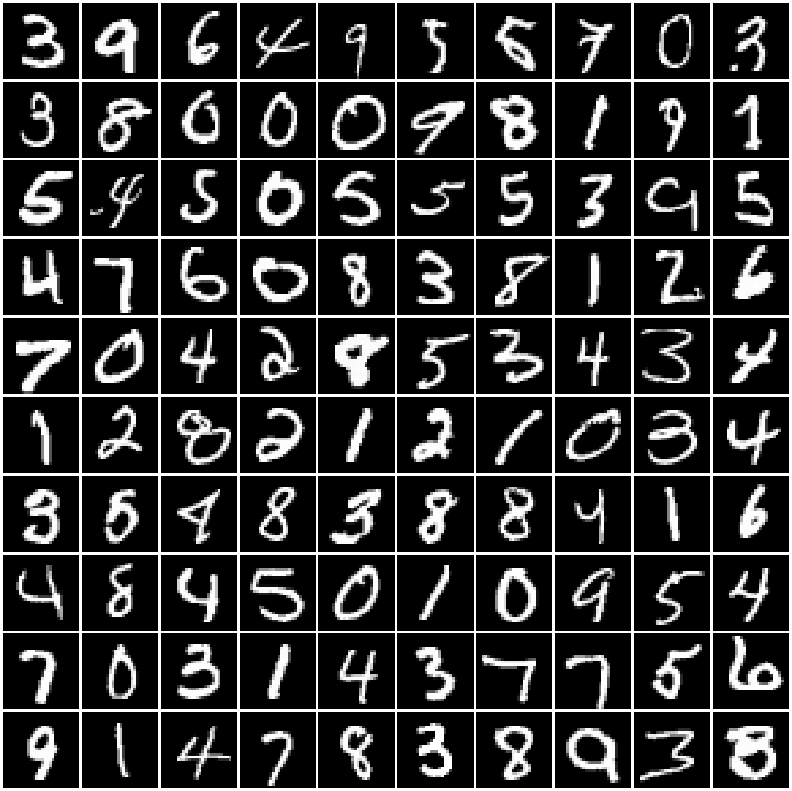
\includegraphics[width=0.40\textwidth]{thesis_data/mnist_example.png}
  \label{fig:MNISTExample}
}
\subfigure[A subsample from the SmallNORB dataset]{
  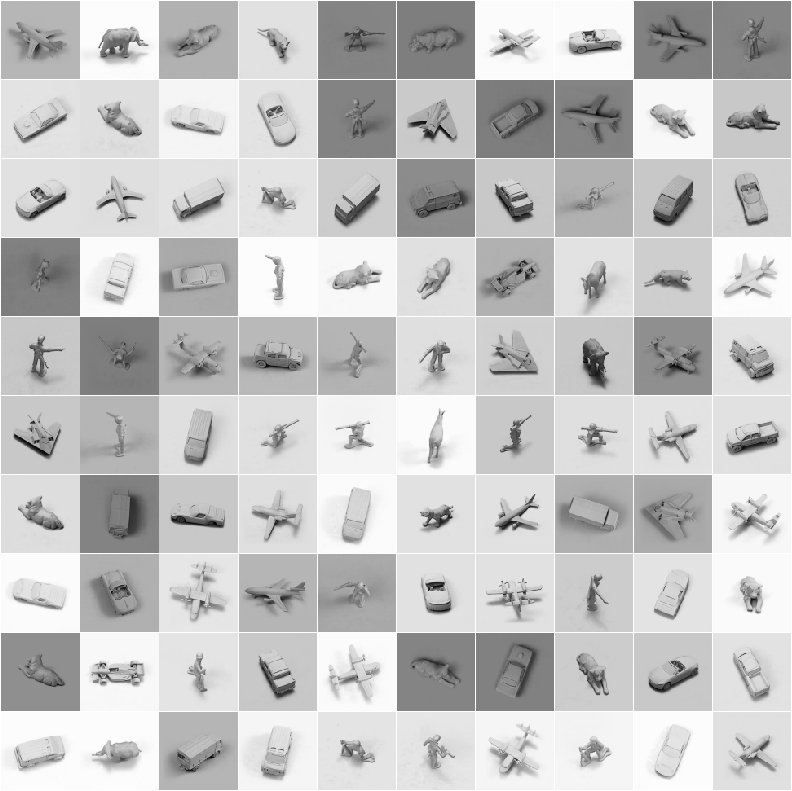
\includegraphics[width=0.40\textwidth]{thesis_data/norbsmall_example.png}
  \label{fig:NORBSmallExample}
}
\subfigure[MNIST patches]{
  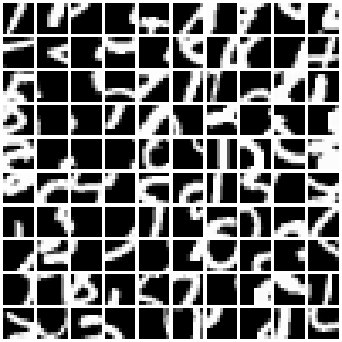
\includegraphics[width=0.40\textwidth]{thesis_data/mnist_patches.png}
  \label{fig:MNISTPatches}
}
\subfigure[SmallNORB patches]{
  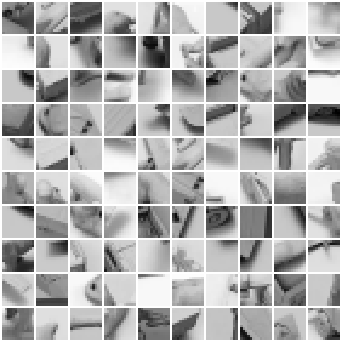
\includegraphics[width=0.40\textwidth]{thesis_data/norbsmall_patches.png}
  \label{fig:NORBSmallPatches}
}
\subfigure[MNIST patches with ZCA applied]{
  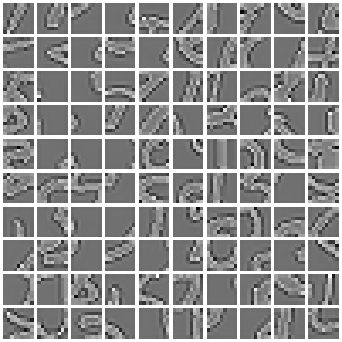
\includegraphics[width=0.40\textwidth]{thesis_data/mnist_patches_zca.png}
  \label{fig:MNISTPatchesZCA}
}
\subfigure[SmallNORB patches widt ZCA applied]{
  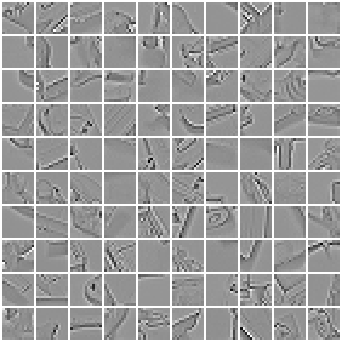
\includegraphics[width=0.40\textwidth]{thesis_data/norbsmall_patches_zca.png}
  \label{fig:NORBSmallPatchesZCA}
}
\caption{Subsamples and patches from MNIST and SmallNORB. The \textbf{ZCA} transformed patches in row three correspond to the original patches in row two.}
\label{fig:ViewsOfMNISTAndNORBSmall}
\end{figure}

\clearpage

\section{Coding, Reconstruction and Sparseness}
\label{sec:CodingReconstructionSparseness}

In this section we will talk again about coding methods, and compare their reconstructive and sparseness inducing powers. A set of $1000$ patches from the SmallNORB dataset will be used for evaluating the different methods. We will work with five feature sets, which we assume are given: a set of $w=169$ random features, a set of $w=169$ \textbf{PCA} features, a set of $w=169$ sparse features, anoter set of $w=512$ random features and another set of $w=512$ sparse features. The first three sets are critically-complete while the last two are roughly three times overcomplete. No overcomplete \textbf{PCA} feature set could, of course, be built. The \textbf{PCA} and sparse $w=169$ sets can be seen in \textbf{Figure \ref{fig:RecSparseFeatureSets}}. The larger sparse feature set is similar to the one shown. The coding methods we are interested in are inner product (\textbf{Corr}), \textbf{MP}, \textbf{OMP}, \textbf{OOMP} and SparseNet with $S(x) = \log(1 + x^2)$.

\begin{figure}
\centering
\subfigure[PCA feature set with $w=169$.]{
  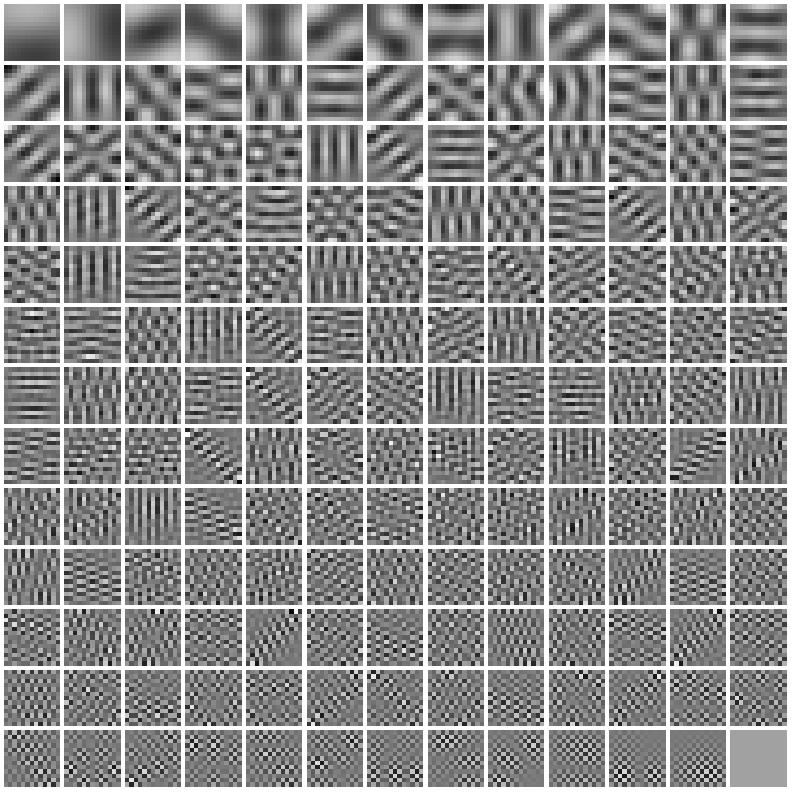
\includegraphics[width=0.45\textwidth]{thesis_data/recsparse/features_pca.png}
  \label{fig:RecSparseFeaturesPCA}
}
\subfigure[Sparse feature set with $w=169$.]{
  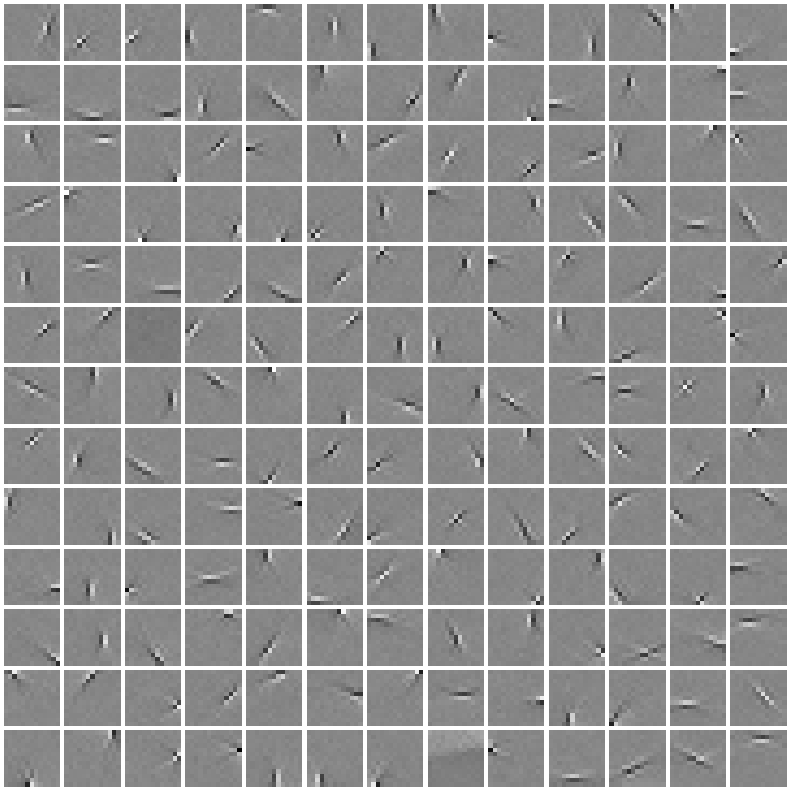
\includegraphics[width=0.45\textwidth]{thesis_data/recsparse/features_sparse.png}
  \label{fig:RecSparseFeaturesSparse}
}
\caption{Two of the three non-random feature sets employed in this section's experiments.}
\label{fig:RecSparseFeatureSets}
\end{figure}

In order to test the reconstruction power of the five coding methods we will measure the average squared sum of differences between an original patch $\textbf{x}$ and a reconstructed patch $\textbf{C}\textbf{a}$. That is, the average Euclidean norm of the error patch $\textbf{x} - \textbf{C}\textbf{a}$. We use the conventions estabilished in the chapter about coding methods. More precisely, $\textbf{C}$ is one of the five feature sets while $\textbf{a}$ is the code word obtained by applying one of the five coding methods we're testing to $\textbf{x}$ and $\textbf{C}$.

For this experiment we will constrain the reconstructive powers of the methods by imposing at most $k$ non-null coefficients. For \textbf{Corr} and SparseNet, the method will be allowed to run as usual, then the $k$ greatest coefficients in absolute value will be selected. \textbf{MP}, \textbf{OMP} and \textbf{OOMP} have $k$ builtin, therefore they suffer no modification. We will have five different values for $k$, namely, $1$, $3$, $16$, $64$ and $w$. When $k=1$ we will have a very strict coding setup. Basically, for a given $\textbf{x}$, $\textbf{a}$ will be zero everywhere except at the index $\omega$ corresponding to the most similar feature from $\textbf{C}$ to $\textbf{x}$. The similarity will be measured by inner-product / projection size of $\textbf{x}$ onto $\textbf{C}^\omega$. We expect \textbf{Corr}, \textbf{MP}, \textbf{OMP} and \textbf{OOMP} to produce the same results, as, for $k=1$, algorithmically speaking, there are no differences between the methods - even the least squares problems \textbf{OMP} and \textbf{OOMP} solve are reduced to inner product comparisons in such a limit case. When $k=3$ we will again have a very strict coding setup, though not as harsh as for $k=1$. We expect large errors in these two situations. For $k=16$ and $k=64$, differences between the methods will start to become apparent and we expect small errors. For $k=w$ we should see in a lot of methods and under a lot of feature sets the error reduced to $0$. For \textbf{OMP} and \textbf{OOMP}, in this case we'll have $k=169$, because, by their very construction, these methods guarantee a $0$ norm residual after $k=d$ steps, therefore every coefficient of $a$ for $t \ge d$ will necessarily be $0$. There is no point in wasting computational resources computing them.

\renewcommand{\arraystretch}{1.2}
\begin{table}
  \caption{Average reconstruction error for different coding methods and different feature sets.}
  \label{table:RecSparseErrors}
  \newcolumntype{R}{>{\centering}X}
  \begin{tabularx}{\textwidth}{|R|R|c|c|c|c|c|}
    \hline
    Features & Method & $k=1$ & $k=3$ & $k=16$ & $k=64$ & $k=w$ \tabularnewline \hline\hline
    \multirow{5}{*}{Random $w=169$} & \textbf{Corr} & $1.95$  & $1.88$ & $1.72$ & $1.81$ & $1.93$ \tabularnewline
    & \textbf{MP} & $1.95$ & $1.87$ & $1.57$ & $1.14$ & $0.87$ \tabularnewline
    & \textbf{OMP} & $1.95$ & $1.87$ & $1.55$ & $0.93$ & $0.00$ \tabularnewline
    & \textbf{OOMP} & $1.95$ & $1.87$ & $1.55$ & $0.93$ & $0.00$ \tabularnewline
    & SparseNet & $1.97$ & $1.93$ & $1.79$ & $1.58$ & $1.50$ \tabularnewline \hline
    \multirow{5}{*}{\textbf{PCA} $w=169$} & \textbf{Corr} & $1.47$ & $1.07$ & $0.55$ & $0.20$ & $0.00$ \tabularnewline
    & \textbf{MP} & $1.47$ & $1.07$ & $0.55$ & $0.20$ & $0.00$ \tabularnewline
    & \textbf{OMP} & $1.47$ & $1.07$ & $0.55$ & $0.20$ & $0.00$ \tabularnewline
    & \textbf{OOMP} & $1.47$ & $1.07$ & $0.55$ & $0.20$ & $0.00$ \tabularnewline
    & SparseNet & $1.58$ & $1.30$ & $1.01$ & $0.91$ & $0.90$ \tabularnewline \hline
    \multirow{5}{*}{Sparse $w=169$} & \textbf{Corr} & $1.76$ & $1.62$ & $1.25$ & $1.03$ & $1.04$ \tabularnewline
    & \textbf{MP} & $1.76$ & $1.61$ & $1.17$ & $0.57$ & $0.16$ \tabularnewline
    & \textbf{OMP} & $1.76$ & $1.61$ & $1.16$ & $0.50$ & $0.00$ \tabularnewline
    & \textbf{OOMP} & $1.76$ & $1.61$ & $1.16$ & $0.50$ & $0.00$ \tabularnewline
    & SparseNet & $1.83$ & $1.74$ & $1.51$ & $1.29$ & $1.24$ \tabularnewline \hline
    \multirow{5}{*}{Random $w=512$} & \textbf{Corr} & $1.93$ & $1.84$ & $1.71$ & $2.59$ & $5.20$ \tabularnewline
    & \textbf{MP} & $1.93$ & $1.83$ & $1.40$ & $0.68$ & $0.01$ \tabularnewline
    & \textbf{OMP} & $1.93$ & $1.83$ & $1.37$ & $0.44$ & $0.00$ \tabularnewline
    & \textbf{OOMP} & $1.93$ & $1.83$ & $1.37$ & $0.43$ & $0.00$ \tabularnewline
    & SparseNet & $1.96$ & $1.93$ & $1.78$ & $1.47$ & $0.89$ \tabularnewline \hline
    \multirow{5}{*}{Sparse $w=512$} & \textbf{Corr} & $1.75$ & $1.62$ & $1.98$ & $3.84$ & $7.02$ \tabularnewline
    & \textbf{MP} & $1.76$ & $1.53$ & $0.99$ & $0.40$ & $0.00$ \tabularnewline
    & \textbf{OMP} & $1.76$ & $1.53$ & $0.95$ & $0.26$ & $0.00$ \tabularnewline
    & \textbf{OOMP} & $1.76$ & $1.53$ & $0.95$ & $0.25$ & $0.00$ \tabularnewline
    & SparseNet & $1.88$ & $1.78$ & $1.56$ & $1.23$ & $0.80$ \tabularnewline \hline
  \end{tabularx}
\end{table}
\renewcommand{\arraystretch}{1.0}

\clearpage

A summary  of the results can be seen in \textbf{Table \ref{table:RecSparseErrors}}. Only the means are presented, however. The variances tended to be the same across methods and feature sets, and were roughly $0.40$ for $k=1$, $k=3$ and $k=16$, $0.10$ for $k=64$ and $0$ for $k=w$, except for SparseNet, which had a $0.10$ variance for this case as well. Several observations need to be made. First, regardless of feature set, reconstruction error goes down from \textbf{Corr} to \textbf{MP} to \textbf{OMP} to \textbf{OOMP}. Furthermore, for \textbf{Corr}, the error increases when  using random features. This breakdown is explained by the nature of the feature set - there is no simple structure to exploit - and the nature of the method - it cannot find ``hidden'' structure. When employing the sparse feature set with $w=169$, which does have some structure to it, the error drops to about half for $k=w$. For the overcomplete sparse set, however, the error radically increases. This is a sign of the severe limitations of the method - even with some structure it cannot produce a suitable approximation when there are more features than dimensions in the signal space. The \textbf{PCA} feature set presents itself in a form which \textbf{Corr} can handle. Therefore, for $k=w$ we have a zero error. More importantly, all methods which are somehow based on inner-products have the same behaviour for this feature set. With regards to inner-product based methods, \textbf{MP} handles itself well. For smaller $k$s it is roughly equivalent to the more complex methods. Better results are obtained in the overcomplete feature sets (both random and sparse) than the critically-complete one. For the overcomplete ones, at $k=512$ a zero error is actually reached. This means the bigger feature set allowed the method a way to find the certain features which allow a perfect reconstruction. The other two methods, \textbf{OMP} and \textbf{OOMP} behave roughly the same. \textbf{OOMP} seems to be a little bit better (by $0.01$ in some cases), but such a small difference would not recommend the method, from a purely approximation power point of view, given its increased compuational demands. As expected, when $k=169$ (the maximum useful for these methods, regardless of the actual $w$), the reconstruction is perfect, regardless of the feature set used. SparseNet does not produce very good approximations. Visual inspection of the result usually hints that there is a scale problem, rather than a shape problem. Also, the overcomplete sparse feature sete is the one which induces best results for this method, although the \textbf{PCA} set is not that far off.

\textbf{Figure \ref{fig:RecSparsePictures}} gives an ideea of the quality of a reconstructed patch, relative to the original. Notice that the patches corresponding to the random bases are more noisy than the other ones and that the patches corresponding to \textbf{PCA} are very similar to the original, regardeless of coding method. Also, the features of the SparseNet patches are barely percievable, even though a closer inspection will reveal the same general shape. This is caused by the previously mentioned amplitude problems.

\begin{figure}
\centering
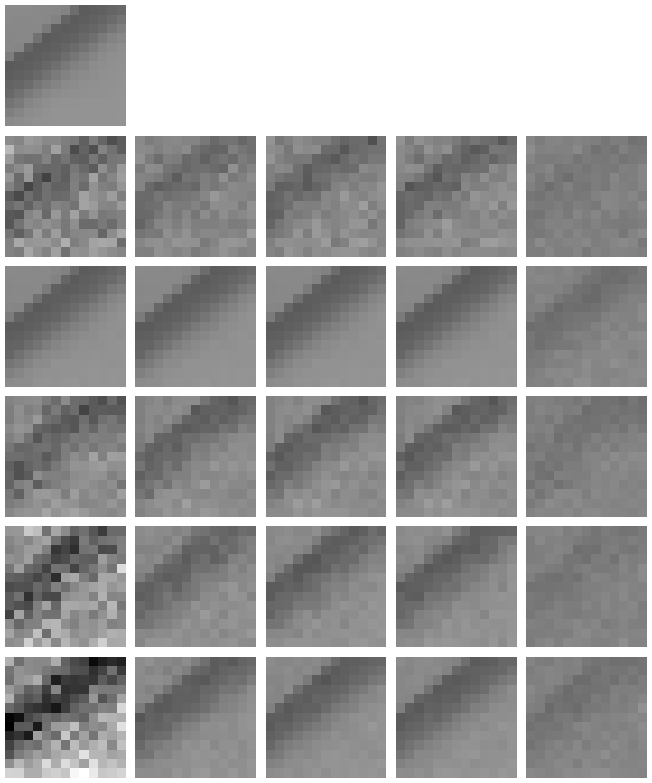
\includegraphics[width=0.95\textwidth,height=0.8\textheight]{thesis_data/recsparse/rec_pictures.png}
\caption{Reconstructions of the patch in the top-left corner using different coding methods and feature sets, but with fixed $k=64$. Each column presents one coding method. They are in order: \textbf{Corr}, \textbf{MP}, \textbf{OMP}, \textbf{OOMP} and SparseNet. Each row, after the first one, presents one feature set. They are in order: random features with $w=169$, \textbf{PCA} features with $w=169$, sparse features with $w=169$, random features with $w=512$ and sparse features with $w=512$.}
\label{fig:RecSparsePictures}
\end{figure}

Reconstruction power is just one measure of the quality of a coding method, however. Another is, of course, sparseness, as measured by the sparseness coefficient $\rho(\textbf{a})$. As in the last experiment, where we were interested in the average reconstruction error, we are now interested in the average sparseness. We continue with the same experimental setup as before. However, we will not impose a small $k$, but rather use $k=w$ or $k=d$, depending on the particular method. Imposing a $k \ll w$ would have artificially restricted the spareness and we would have gotten useful results only for larger values of $k$, for which the methods would be able to induce their own spareness. We use a $\delta = 0.01$ as the threshold value for a coefficient being close to zero in the computation of the sparseness coefficient.

\renewcommand{\arraystretch}{1.2}
\begin{table}
  \caption{Average sparseness for different coding methods and different feature sets.}
  \label{table:RecSparseSparseness}
  \newcolumntype{R}{>{\centering}X}
  \begin{tabularx}{\textwidth}{|R|c|c|c|c|c|}
    \hline
    Features & \textbf{Corr} & \textbf{MP} & \textbf{OMP} & \textbf{OOMP} & SparseNet \tabularnewline \hline\hline
    Random $w=169$ & $0.48$ & $0.50$ & $0.50$ & $0.50$ & $0.41$ \tabularnewline \hline
    \textbf{PCA} $w=169$ & $0.36$ & $0.36$ & $0.36$ & $0.36$ & $0.38$ \tabularnewline \hline
    Sparse $w=169$ & $0.46$ & $0.50$ & $0.45$ & $0.45$ & $0.42$ \tabularnewline \hline
    Random $w=512$ & $0.47$ & $0.28$ & $0.13$ & $0.13$ & $0.37$ \tabularnewline \hline
    Sparse $w=512$ & $0.47$ & $0.19$ & $0.12$ & $0.12$ & $0.35$ \tabularnewline
    \hline
  \end{tabularx}
\end{table}
\renewcommand{\arraystretch}{1.0}

A summary of the results can be seen in \textbf{Table \ref{table:RecSparseSparseness}}. For the critically-complete random feature set every inner-product bases method performs roughly the same. SparseNet is significantly better, though, in general, all methods perform rather poorly, requiring about half of the coefficients to be greater than $\delta$. With \textbf{PCA} features, we again see the identical behaviour for all inner-product based methods. All methods have roughly the same behaviour, which is visibly better than with the random features, but not that great in general. Similarly, with the critically-complete sparse feature set, about half of the code word coefficients are active, regardless of method. However, \textbf{MP} is a little bit worse than \textbf{Corr} and the other pursuits. It probably can't find good matches in this limited feature set. SparseNet again leads the pack with performance similar to the random feature set case. When we move to the larger feature sets, however, the situation changes drastically. \textbf{Corr} remains at roughly the same level as with the $w=169$ feature sets, and SparseNet is slighly better, but the pursuits come into their own and produce very sparse results. Again, \textbf{OMP} and \textbf{OOMP} produce ``identical'' results, furthering our belief that the second has no practical advantage over the first. \textbf{MP} is roughly half as good as \textbf{OMP} and \textbf{OOMP}, especially in the random feature set, but is much better than simple correlation. Notice that, in absolute terms, in the best cases, roughly $60$ coefficients are needed for a good reconstruction, as $\hctimes{0.50}{128} \approx \hctimes{0.12}{512} \approx 60$. This is useful information for later experiments. Using a $k > 60$ with a $d$ similar to the ones we used in these experiments, will, most likely, not produce better results.

\begin{figure}
\centering
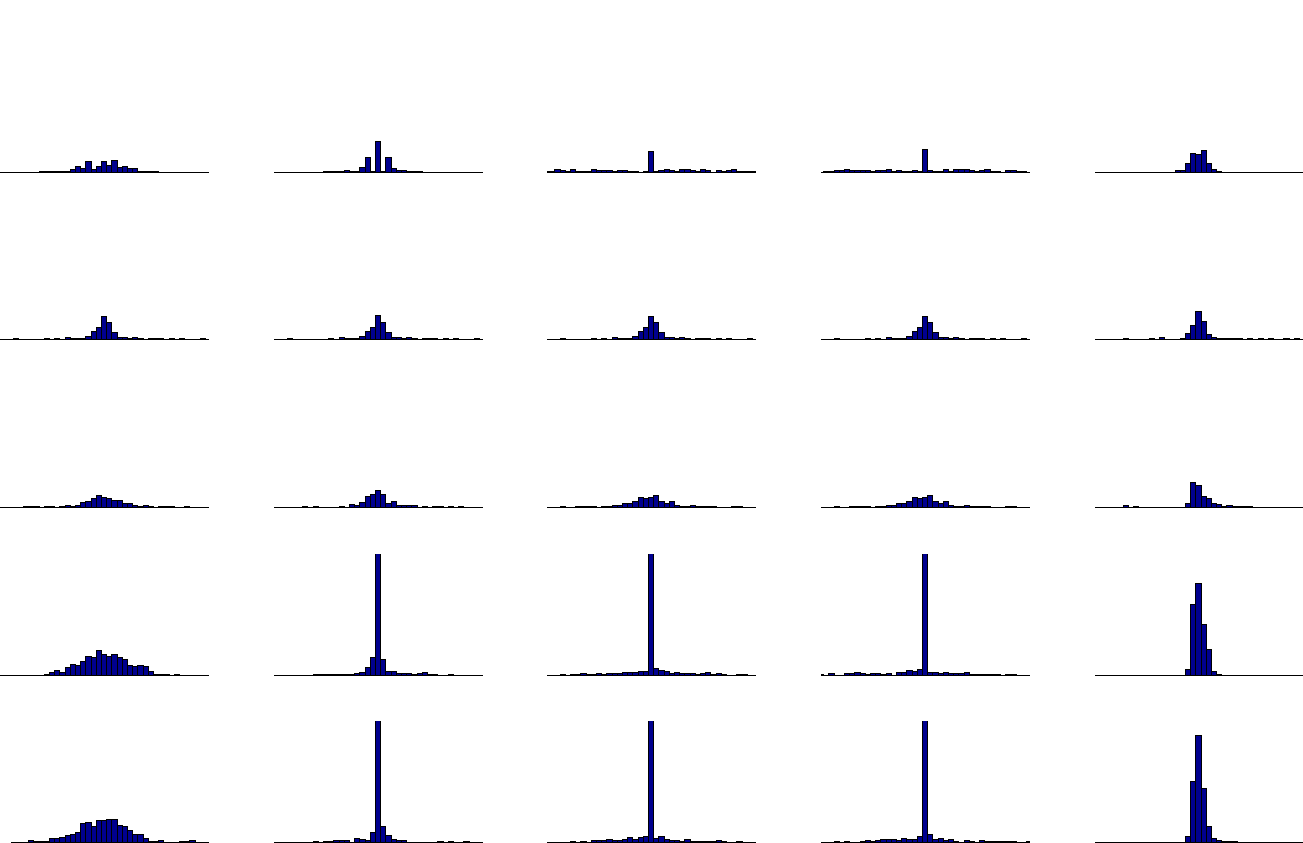
\includegraphics[width=0.95\textwidth,height=0.8\textheight]{thesis_data/recsparse/rec_hists.png}
\caption{Histograms of the code words for the patch in the top-left corner of \textbf{Figure \ref{fig:RecSparsePictures}} produced using different coding methods and feature sets. Each columns presents one coding method. They are in order: \textbf{Corr}, \textbf{MP}, \textbf{OMP}, \textbf{OOMP} and SparseNet. Each row presents one feature set. They are in order: random features with $w=169$, \textbf{PCA} features with $w=169$, sparse features with $w=169$, random features with $w=512$ and sparse features with $w=512$. All horizontal axes are between $[-1.5,1.5]$ and all vertical ones are between $[0,250]$.}
\label{fig:RecSparseHists}
\end{figure}

\textbf{Figure \ref{fig:RecSparseHists}} gives an ideea of the distribution of the patches in the different cases. We used $61$ bins spread evenly in the interval $[-1.5,1.5]$. Notice how spiked the distributions for the pursuits are, expecially for \textbf{OMP} and \textbf{OOMP}. Again, these two produce almost identical results. The distribution for \textbf{Corr} is however very flat. \textbf{MP} is situated somewhat between these two extremes, but with a clear peak around $0$. Similarly, SparseNet has a peak around $0$, but the distribution has a skwed form, resulting from the regularization term we used. The effect is good, although the sparsity is clearly more strinking in the \textbf{OMP} and \textbf{OOMP} methods. The \textbf{PCA} features do not produce very ``sparse'' looking histograms, regardless of the methods employed, despite good reconstruction performance and acceptable average sparseness. Real sparseness is to be found in the way the values are distributed - there must be just a few code word coefficients with large values, besides being a lot of them equal to or near $0$.

\section{Learning Sparse Feature Sets}
\label{sec:LearningSparseFeatureSet}

[[[We have to see about what we'll talk about in this section.]]]

\section{Coder Architecture Evaluation}
\label{sec:CoderArchitectureEvaluation}

[[[Show link reconstruction power and classification accuracy]]]

In this section we will seek the best coder architectures for the image classification tasks posed by the MNIST and SmallNORB datasets, described in the start of this chapter. We will use the feature extractor model described in \textbf{Chapter \ref{chap:OverviewFeatureExtraction}}, and, as mentioned there, we will employ just one recoder module. Given a certain problem, the task is to pick the recoder parameters in such a way as to maximize the classification accuracy on the test version of the dataset. The recoder parameters are the parameters for each of the four stages. For the coding stage we have the feature size $d = \hctimes{p}{p}$, the feature set $\textbf{C}$ and $w$, the number of allowed non-small coefficients $k$ and the actual coding method $\mathcal{C}_{\textbf{C},k}$. For the nonlinear step we have the nonlinearity type $\mathcal{N}$. For the polarity split stage we have the split type $\mathcal{P}$. Finally, for the reduce step we have the reducer procedure $\mathcal{R}$ and the size of the spread $r$. Instead of $k$ we will use $\hat{\rho} = k/w$. This makes it somewhat easier to compare parameter sets, independent of $w$. Thus, a full parameterization of the recoder is $(p,w,\textbf{C},\hat{\rho},\mathcal{C}_{\textbf{C},k},\mathcal{N},\mathcal{P},\mathcal{R},r)$.

\begin{wrapfigure}{R}{0.25\textwidth}
\begin{center}
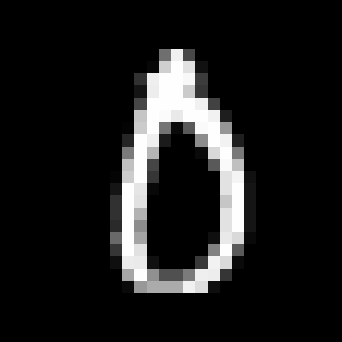
\includegraphics[width=0.25\textwidth]{thesis_data/recoderev/original_image.png}
\end{center}
\caption{The original image which is coded in \textbf{Figure \ref{fig:RecoderEvRecodingExamplesCorr}} and \textbf{Figure \ref{fig:RecoderEvRecodingExamplesOOMP}}.}
\label{fig:RecoderEvOriginalImage}
\end{wrapfigure}

Before we describe the experiments performed and the results obtained, \textbf{Figure \ref{fig:RecoderEvRecodingExamplesCorr}} and \textbf{Figure \ref{fig:RecoderEvRecodingExamplesOOMP}} show how the image in \textbf{Figure \ref{fig:RecoderEvOriginalImage}} looks after recoding. For both image sets, a very small feature set of $w=9$ patches of size $\hctimes{9}{9}$ were used, for illustrative purposes. The coded output is a vector of size $\lfloor m / r \rfloor \lfloor n / r \rfloor w$ which can be interpreted as a series of $w$ $\hctimes{\lfloor m / r \rfloor}{\lfloor n / r \rfloor}$ images - a three dimensional tensor. Each image is associated with a single feature and represents the original image coded with regards to that feature. As we mentioned earlier, in the most general case, the coefficients in one image depend on the corresponding coefficients in the other images. In any case, this form is good for visualizing how the different architecture choices influence the coded output. The images are displayed in the odd rows, and as a vector in the even rows. Notice that, in order to go from the tensor representation to the linear one, no transformations need be applied, as, in our implementation, the data is stored in the proper order. Therefore, the first coefficients of the linear form correspond to the first image, the next coefficients correspond to the second image etc. When polarity splitting is used, the positive coefficients appear in the first half of the liner form, while the negative coefficients appear in the second half. The order in these two regions is the same as in the case of no polarity splitting.

\begin{figure}
\centering
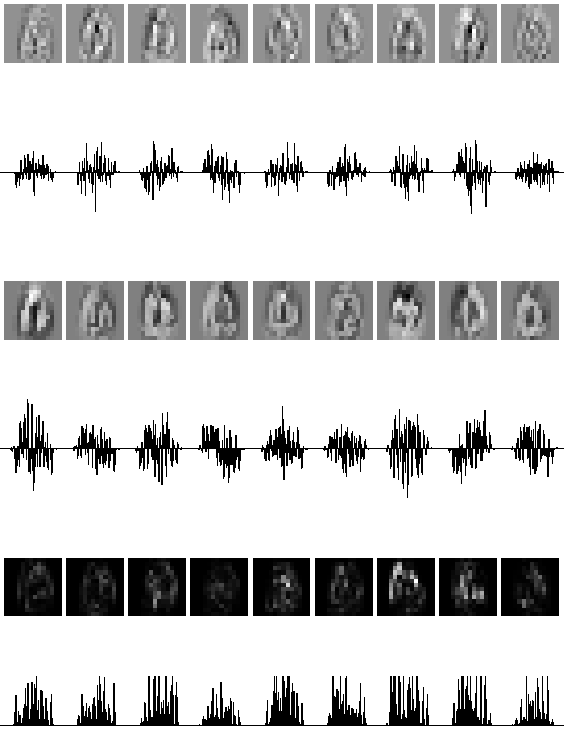
\includegraphics[width=0.95\textwidth,height=0.8\textheight]{thesis_data/recoderev/coded_partial_corr.png}
\caption{Different views of the coded image in \textbf{Figure \ref{fig:RecoderEvOriginalImage}}. The coding was done with the \textbf{Corr} coding method. The odd rows present the code word coefficients for each one of th e $w=9$ features, arranged as an image. The even rows present the actual ``linear'' form of the recoded image, which is fed to a classifier, for example. The row pairs are, in order: linear nonlinearity, no polarity split, subsample reduce; linear nonlinearity, no polarity split, maximum with sign kept reduce; linear nonlinearity, no polarity split, sum of squares reduce. See the text for more details.}
\label{fig:RecoderEvRecodingExamplesCorr}
\end{figure}

\begin{figure}
\centering
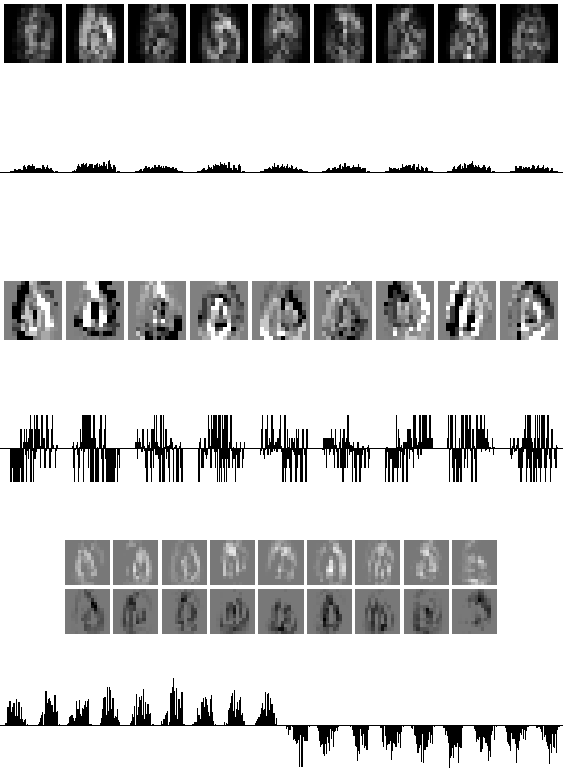
\includegraphics[width=0.95\textwidth,height=0.8\textheight]{thesis_data/recoderev/coded_partial_oomp.png}
\caption{Different views of the coded image in \textbf{Figure \ref{fig:RecoderEvOriginalImage}}. The coding was done with the \textbf{OOMP} coding method. The odd rows present the code word coefficients for each one of th e $w=9$ features, arranged as an image. The even rows present the actual ``linear'' form of the recoded image, which is fed to a classifier, for example. The row pairs are, in order: logistic nonlinearity, no polarity split, maximum with no sign kept reduce; global order nonlinearity, no polarity split, maximum with sign reduce; linear nonlinearity, polarity split with kept sign, maximum with kept sign reduce. See the text for more details.}
\label{fig:RecoderEvRecodingExamplesOOMP}
\end{figure}

\renewcommand{\arraystretch}{1.5}
\begin{table}
  \caption{Allowed values for the recoder parameters.}
  \label{table:RecoderEvAllowedParams}
  \newcolumntype{R}{>{\centering}X}
  \begin{tabularx}{\textwidth}{|c|R|}
    \hline
    Parameter & Allowed values \tabularnewline \hline\hline
    $p$ & $5,7,9,11,13,15,17$ \tabularnewline \hline
    $w$ & $p^2,3p^2$ and $1024,1536,2048$ \tabularnewline \hline
    $\textbf{C}$ & Random, \textbf{PCA}, Sparse \tabularnewline \hline
    $\hat{\rho} = k / w$ & $0.05,0.10,\dots,0.45,0.50$ \tabularnewline \hline
    $\mathcal{C}_{\textbf{C},k}$ & \textbf{Corr}, \textbf{MP}, \textbf{OMP}, \textbf{OOMP} \tabularnewline \hline
    $\mathcal{N}$ & Linear, Logistic, GlobalOrder \tabularnewline \hline
    $\mathcal{P}$ & None, NoSign, KeepSign \tabularnewline \hline
    $\mathcal{R}$ & Subsample, MaxNoSign, MaxKeepSign, SumAbs, SumSqr \tabularnewline \hline
    $r$ & $2,3,4,6,8,10,14,20$ \tabularnewline
    \hline
  \end{tabularx}
\end{table}
\renewcommand{\arraystretch}{1.0}

Returning to our experiment, we can see in \textbf{Table \ref{table:RecoderEvAllowedParams}} a list of possible values for all the different parameters associated with a recoder, usable by both datasets. An exhaustive search of the full parameter space would require evaluating almost $5$ million different parameter combinations - clearly a very hard task! The only way forward is to manage this complexity. One approach for doing this, is to split the problem into several subproblems which are ``independent'' enough. The best configuration is then formed by combining the answers to the subproblems. One thing we'll need is an initial ``good-enough'' parameter set. \textbf{Table \ref{table:RecoderEvInitialConfigs}} presents not one, but two such configurations, dubbed $\Theta_1^0$,$\Theta_2^0$ and $\Theta_3^0$, which have been obtained through trial and error and eariler undocumented experiments. The subproblems will try to improve upon these three initial configurations.

\renewcommand{\arraystretch}{1.2}
\begin{table}
  \caption{Initial ``good'' configurations.}
  \label{table:RecoderEvInitialConfigs}
  \newcolumntype{R}{>{\centering}X}
  \begin{tabularx}{\textwidth}{|R|ccccccccccc|}
    \hline
     & $p$ & $w$ & $\textbf{C}$ & $\hat{\rho}$ & $\mathcal{C}_{\textbf{C},k}$ & $\mathcal{N}$ & $\mathcal{P}$ & $\mathcal{R}$ & $r$ & Score & $\mathbb{E}[\rho]$ \tabularnewline\hline\hline
    $\Theta_1^0$ & $11$ & $3p^2$ & Sparse & $0.10$ & \textbf{MP} & Logistic & None & SumSqr & $4$ & $\textbf{99.06}$ & $0.26$ \tabularnewline
    $\Theta_2^0$ & $11$ & $3p^2$ & Random & $0.10$ & \textbf{Corr} & Global & None & SumSqr & $4$ & $\textbf{99.28}$ & $0.31$ \tabularnewline
    $\Theta_3^0$ & $11$ & $2p^2$ & Sparse & $0.10$ & \textbf{OMP} & Logistic & KeepSign & SumSqr & $4$ & $\textbf{99.13}$ & $0.20$ \tabularnewline
    \hline
  \end{tabularx}
\end{table}
\renewcommand{\arraystretch}{1.0}

We split the parameter set into three groups: feature set parameters ($p$,$w$ and $\textbf{C}$), coding method parameters ($\hat{\rho}$ and $\mathcal{C}_{\textbf{C},k}$) and aftercoding stage parameters ($\mathcal{N}$, $\mathcal{P}$, $\mathcal{R}$ and $r$). The subproblems will then handle each of these three parameter sets sperately. More precisely, the following procedure will be followed. Every combination of feature set parameters from \textbf{Table \ref{table:RecoderEvAllowedParams}} is used, except the $w$s which are over $1000$. More precisely, for every $p$ tested we use a critically-complete feature set and a double overcomplete feature set. We do not use feature sets of a higher count because of computational concerns. There are nine distinct values for $p$, two values for $w$ and three values for \textbf{C}. Therefore we can form $90$ different parameter combinations. For each test, the other parameters come from $\Theta_1^0$, $\Theta_2^0$ and $\Theta_3^0$ respectively. Therefore, we will test a total of $270$ full parameter combinations. After this first experiment, we select the three best full parameter configurations and name them $\Theta_1^1$, $\Theta_2^1$ and $\Theta_3^1$. We then continue with the second experiment, which looks at every combination of coding method parameters from \textbf{Table \ref{table:RecoderEvAllowedParams}}. There are twenty distinct values for $\hat{\rho}$ and three distinct values for $\mathcal{C}_{\textbf{C},k}$. Therefore we can form $60$ different parameter combinations. For each test, the other parameters come from $\Theta_1^1$, $\Theta_2^1$ and $\Theta_3^1$ respectively. Therefore, we will test a total of $180$ full parameter combinations. After this second experiment, we select the three best full parameter configurations and name them $\Theta_1^2$, $\Theta_2^2$ and $\Theta_3^2$. We then continue with the third experiment, which looks at every combination of parameters for all the stages after the coding stage. There are three distinct values for $\mathcal{N}$, three distinct values for $\mathcal{R}$, five distinct values for $\mathcal{R}$ and eight distinct values for $r$. Therefore, we can form $360$ different parameter combinations. For each test, the other parameters come from $\Theta_1^2$, $\Theta_2^2$ and $\Theta_3^2$ respectively. Therefore we will test a total of $1080$ full parameter combinations. After this third experiment, we select the three best full parameter configurations and name them $\Theta_1^3$, $\Theta_2^3$ and $\Theta_3^3$. As a final experiment we will look at how these three configurations perform with very high $w$ and varying $\hat{\rho}$.

\renewcommand{\arraystretch}{1.2}
\begin{table}
  \caption{Summarized experiment results for MNIST.}
  \label{table:RecoderEvMNISTResultsSummarized}
  \newcolumntype{R}{>{\centering}X}
  \begin{tabularx}{\textwidth}{|R|ccccccccccc|}
    \hline
    & $p$ & $w$ & $\textbf{C}$ & $\hat{\rho}$ & $\mathcal{C}_{\textbf{C},k}$ & $\mathcal{N}$ & $\mathcal{P}$ & $\mathcal{R}$ & $r$ & Score & $\mathbb{E}[\rho]$ \tabularnewline\hline\hline
    $\Theta_1^1$ & $11$ & $3p^2$ & Random & $0.10$ & \textbf{Corr} & Global & None & SumSqr & $4$ & x & x \tabularnewline
    $\Theta_2^1$ & $15$ & $3p^2$ & Random & $0.10$ & \textbf{Corr} & Global & None & SumSqr & $4$ & x & x \tabularnewline
    $\Theta_3^1$ & $13$ & $3p^2$ & Sparse & $0.10$ & \textbf{OMP} & Logistic & KeepSign & SumSqr & $4$ & x & x \tabularnewline\hline\hline
    $\Theta_1^2$ & $11$ & $256$ & Sparse & $0.10$ & \textbf{MP} & Logistic & None & SumSqr & $4$ & 98.50 & 0.11 \tabularnewline
    $\Theta_2^2$ & $11$ & $256$ & Random & $0.10$ & \textbf{Corr} & Global & None & SumSqr & $4$ & 98.50 & 0.11 \tabularnewline
    $\Theta_3^2$ & $11$ & $256$ & Random & $0.10$ & \textbf{Corr} & Global & None & SumSqr & $4$ & 98.50 & 0.11 \tabularnewline\hline\hline
    $\Theta_1^3$ & $11$ & $256$ & Sparse & $0.10$ & \textbf{MP} & Logistic & None & SumSqr & $4$ & 98.50 & 0.11 \tabularnewline
    $\Theta_2^3$ & $11$ & $256$ & Random & $0.10$ & \textbf{Corr} & Global & None & SumSqr & $4$ & 98.50 & 0.11 \tabularnewline
    $\Theta_3^3$ & $11$ & $256$ & Random & $0.10$ & \textbf{Corr} & Global & None & SumSqr & $4$ & 98.50 & 0.11 \tabularnewline
    \hline
  \end{tabularx}
\end{table}
\renewcommand{\arraystretch}{1.0}

\renewcommand{\arraystretch}{1.2}
\begin{table}
  \caption{Classification scores for first experiments on MNIST.}
  \label{table:RecoderEvMNISTResultsPWCScore}
  \newcolumntype{R}{>{\centering}X}
  \begin{tabularx}{\textwidth}{ccRR|ccccccc|}
    \cline{5-11}
    & & & & \multicolumn{7}{c|}{$p$} \tabularnewline \cline{5-11}
    & & & & $5$ & $7$ & $9$ & $11$ & $13$ & $15$ & $17$ \tabularnewline\hline
    \multicolumn{1}{|c}{\multirow{5}{*}{$\Theta_1^0$}} & \multicolumn{1}{|c}{\multirow{5}{*}{$\textbf{C}$}} & \multicolumn{1}{|R}{\multirow{2}{*}{Random}} & \multicolumn{1}{|R|}{$w=p^2$} & $98.41$ & $98.45$ & $98.64$ & $98.69$ & $98.68$ & $98.62$ & $98.56$ \tabularnewline
    \multicolumn{1}{|c}{} & \multicolumn{1}{|c}{} & \multicolumn{1}{|R}{} & \multicolumn{1}{|R|}{$w=3p^2$} & $98.46$ & $98.62$ & $98.81$ & $98.85$ & $98.77$ & $98.76$ & $98.68$ \tabularnewline
    \multicolumn{1}{|c}{} & \multicolumn{1}{|c}{} & \multicolumn{1}{|R}{\textbf{PCA}} & \multicolumn{1}{|R|}{$w=p^2$} & $98.01$ & $98.15$ & $98.30$ & $98.50$ & $98.52$ & $98.52$ & $98.49$ \tabularnewline
    \multicolumn{1}{|c}{} & \multicolumn{1}{|c}{} & \multicolumn{1}{|R}{\multirow{2}{*}{Sparse}} & \multicolumn{1}{|R|}{$w=p^2$} & $98.04$ & $98.25$ & $98.46$ & $98.54$ & $98.62$ & $98.71$ & $98.73$ \tabularnewline
    \multicolumn{1}{|c}{} & \multicolumn{1}{|c}{} & \multicolumn{1}{|R}{} & \multicolumn{1}{|R|}{$w=3p^2$} & $98.23$ & $98.32$ & $98.51$ & $98.50$ & $98.59$ & $98.73$ & $98.87$ \tabularnewline\hline\hline
    \multicolumn{1}{|c}{\multirow{5}{*}{$\Theta_2^0$}} & \multicolumn{1}{|c}{\multirow{5}{*}{$\textbf{C}$}} & \multicolumn{1}{|R}{\multirow{2}{*}{Random}} & \multicolumn{1}{|R|}{$w=p^2$} & $97.91$ & $98.28$ & $98.68$ & $98.82$ & $98.87$ & $98.91$ & $98.89$ \tabularnewline
    \multicolumn{1}{|c}{} & \multicolumn{1}{|c}{} & \multicolumn{1}{|R}{} & \multicolumn{1}{|R|}{$w=3p^2$} & $98.24$ & $98.62$ & $98.85$ & $\textbf{98.95}$ & $98.88$ & $\textbf{98.99}$ & $98.95$ \tabularnewline
    \multicolumn{1}{|c}{} & \multicolumn{1}{|c}{} & \multicolumn{1}{|R}{\textbf{PCA}} & \multicolumn{1}{|R|}{$w=p^2$} & $97.42$ & $97.82$ & $98.21$ & $98.31$ & $98.32$ & $98.51$ & $98.54$ \tabularnewline
    \multicolumn{1}{|c}{} & \multicolumn{1}{|c}{} & \multicolumn{1}{|R}{\multirow{2}{*}{Sparse}} & \multicolumn{1}{|R|}{$w=p^2$} & $97.52$ & $97.85$ & $98.29$ & $98.54$ & $98.56$ & $98.77$ & $98.78$ \tabularnewline
    \multicolumn{1}{|c}{} & \multicolumn{1}{|c}{} & \multicolumn{1}{|R}{} & \multicolumn{1}{|R|}{$w=3p^2$} & $97.96$ & $97.94$ & $98.25$ & $98.28$ & $98.38$ & $98.52$ & $98.68$ \tabularnewline\hline\hline
    \multicolumn{1}{|c}{\multirow{5}{*}{$\Theta_3^0$}} & \multicolumn{1}{|c}{\multirow{5}{*}{$\textbf{C}$}} & \multicolumn{1}{|R}{\multirow{2}{*}{Random}} & \multicolumn{1}{|R|}{$w=p^2$} & $98.62$ & $98.62$ & $98.68$ & $98.71$ & $98.63$ & $98.64$ & $98.55$ \tabularnewline
    \multicolumn{1}{|c}{} & \multicolumn{1}{|c}{} & \multicolumn{1}{|R}{} & \multicolumn{1}{|R|}{$w=3p^2$} & $98.65$ & $98.77$ & $98.83$ & $98.84$ & $98.74$ & $98.76$ & $98.60$ \tabularnewline
    \multicolumn{1}{|c}{} & \multicolumn{1}{|c}{} & \multicolumn{1}{|R}{\textbf{PCA}} & \multicolumn{1}{|R|}{$w=p^2$} & $98.07$ & $98.24$ & $98.44$ & $98.54$ & $98.48$ & $98.47$ & $98.38$ \tabularnewline
    \multicolumn{1}{|c}{} & \multicolumn{1}{|c}{} & \multicolumn{1}{|R}{\multirow{2}{*}{Sparse}} & \multicolumn{1}{|R|}{$w=p^2$} & $98.33$ & $98.57$ & $98.73$ & $98.80$ & $98.87$ & $98.82$ & $98.88$ \tabularnewline
    \multicolumn{1}{|c}{} & \multicolumn{1}{|c}{} & \multicolumn{1}{|R}{} & \multicolumn{1}{|R|}{$w=3p^2$} & $98.50$ & $98.63$ & $98.59$ & $98.68$ & $\textbf{98.89}$ & $98.86$ & $98.80$ \tabularnewline\hline
  \end{tabularx}
\end{table}
\renewcommand{\arraystretch}{1.0}

\renewcommand{\arraystretch}{1.2}
\begin{table}
  \caption{Classification scores for second experiment on MNIST.}
  \label{table:RecoderEvMNISTResultsRhoCCkScore}
  \newcolumntype{R}{>{\centering}X}
  \begin{tabularx}{\textwidth}{cccc|RRRRR|}
    \cline{5-9}
    & & & & \multicolumn{5}{c|}{$\hat{\delta}$} \tabularnewline\cline{5-9}
    & & & & $0.00$ & $0.05$ & $0.10$ & $0.15$ & $0.20$ \tabularnewline\hline
    \multicolumn{1}{|c}{\multirow{8}{*}{$\Theta_1^1$}} & \multicolumn{1}{|c|}{\multirow{8}{*}{$\mathcal{C}_{\textbf{C},k}$}} & \multirow{2}{*}{\textbf{Corr}} & \multicolumn{1}{|c|}{$\hat{\rho}=0.05+\hat{\delta}$} & $x^1$ & $x^1$ & $x^1$ & $x^1$ & $x^1$ \tabularnewline
    \multicolumn{1}{|c}{} & \multicolumn{1}{|c|}{} & & \multicolumn{1}{|c|}{$\hat{\rho} = 0.25 + \hat{\delta}$} & $x^1$ & $x^1$ & $x^1$ & $x^1$ & $x^1$ \tabularnewline
    \multicolumn{1}{|c}{} & \multicolumn{1}{|c|}{} & \multirow{2}{*}{\textbf{MP}} & \multicolumn{1}{|c|}{$\hat{\rho}=0.05+\hat{\delta}$} & $x^1$ & $x^1$ & $x^1$ & $x^1$ & $x^1$ \tabularnewline
    \multicolumn{1}{|c}{} & \multicolumn{1}{|c|}{} & & \multicolumn{1}{|c|}{$\hat{\rho} = 0.25 + \hat{\delta}$} & $x^1$ & $x^1$ & $x^1$ & $x^1$ & $x^1$ \tabularnewline
    \multicolumn{1}{|c}{} & \multicolumn{1}{|c|}{} & \multirow{2}{*}{\textbf{OMP}} & \multicolumn{1}{|c|}{$\hat{\rho}=0.05+\hat{\delta}$} & $x^1$ & $x^1$ & $x^1$ & $x^1$ & $x^1$ \tabularnewline
    \multicolumn{1}{|c}{} & \multicolumn{1}{|c|}{} & & \multicolumn{1}{|c|}{$\hat{\rho} = 0.25 + \hat{\delta}$} & $x^1$ & $x^1$ & $x^1$ & $x^1$ & $x^1$ \tabularnewline
    \multicolumn{1}{|c}{} & \multicolumn{1}{|c|}{} & \multirow{2}{*}{\textbf{OOMP}} & \multicolumn{1}{|c|}{$\hat{\rho}=0.05+\hat{\delta}$} & $x^1$ & $x^1$ & $x^1$ & $x^1$ & $x^1$ \tabularnewline
    \multicolumn{1}{|c}{} & \multicolumn{1}{|c|}{} & & \multicolumn{1}{|c|}{$\hat{\rho} = 0.25 + \hat{\delta}$} & $x^1$ & $x^1$ & $x^1$ & $x^1$ & $x^1$ \tabularnewline\hline\hline
    \multicolumn{1}{|c}{\multirow{8}{*}{$\Theta_2^1$}} & \multicolumn{1}{|c|}{\multirow{8}{*}{$\mathcal{C}_{\textbf{C},k}$}} & \multirow{2}{*}{\textbf{Corr}} & \multicolumn{1}{|c|}{$\hat{\rho}=0.05+\hat{\delta}$} & $x^1$ & $x^1$ & $x^1$ & $x^1$ & $x^1$ \tabularnewline
    \multicolumn{1}{|c}{} & \multicolumn{1}{|c|}{} & & \multicolumn{1}{|c|}{$\hat{\rho} = 0.25 + \hat{\delta}$} & $x^1$ & $x^1$ & $x^1$ & $x^1$ & $x^1$ \tabularnewline
    \multicolumn{1}{|c}{} & \multicolumn{1}{|c|}{} & \multirow{2}{*}{\textbf{MP}} & \multicolumn{1}{|c|}{$\hat{\rho}=0.05+\hat{\delta}$} & $x^1$ & $x^1$ & $x^1$ & $x^1$ & $x^1$ \tabularnewline
    \multicolumn{1}{|c}{} & \multicolumn{1}{|c|}{} & & \multicolumn{1}{|c|}{$\hat{\rho} = 0.25 + \hat{\delta}$} & $x^1$ & $x^1$ & $x^1$ & $x^1$ & $x^1$ \tabularnewline
    \multicolumn{1}{|c}{} & \multicolumn{1}{|c|}{} & \multirow{2}{*}{\textbf{OMP}} & \multicolumn{1}{|c|}{$\hat{\rho}=0.05+\hat{\delta}$} & $x^1$ & $x^1$ & $x^1$ & $x^1$ & $x^1$ \tabularnewline
    \multicolumn{1}{|c}{} & \multicolumn{1}{|c|}{} & & \multicolumn{1}{|c|}{$\hat{\rho} = 0.25 + \hat{\delta}$} & $x^1$ & $x^1$ & $x^1$ & $x^1$ & $x^1$ \tabularnewline
    \multicolumn{1}{|c}{} & \multicolumn{1}{|c|}{} & \multirow{2}{*}{\textbf{OOMP}} & \multicolumn{1}{|c|}{$\hat{\rho}=0.05+\hat{\delta}$} & $x^1$ & $x^1$ & $x^1$ & $x^1$ & $x^1$ \tabularnewline
    \multicolumn{1}{|c}{} & \multicolumn{1}{|c|}{} & & \multicolumn{1}{|c|}{$\hat{\rho} = 0.25 + \hat{\delta}$} & $x^1$ & $x^1$ & $x^1$ & $x^1$ & $x^1$ \tabularnewline\hline\hline
    \multicolumn{1}{|c}{\multirow{8}{*}{$\Theta_3^1$}} & \multicolumn{1}{|c|}{\multirow{8}{*}{$\mathcal{C}_{\textbf{C},k}$}} & \multirow{2}{*}{\textbf{Corr}} & \multicolumn{1}{|c|}{$\hat{\rho}=0.05+\hat{\delta}$} & $x^1$ & $x^1$ & $x^1$ & $x^1$ & $x^1$ \tabularnewline
    \multicolumn{1}{|c}{} & \multicolumn{1}{|c|}{} & & \multicolumn{1}{|c|}{$\hat{\rho} = 0.25 + \hat{\delta}$} & $x^1$ & $x^1$ & $x^1$ & $x^1$ & $x^1$ \tabularnewline
    \multicolumn{1}{|c}{} & \multicolumn{1}{|c|}{} & \multirow{2}{*}{\textbf{MP}} & \multicolumn{1}{|c|}{$\hat{\rho}=0.05+\hat{\delta}$} & $x^1$ & $x^1$ & $x^1$ & $x^1$ & $x^1$ \tabularnewline
    \multicolumn{1}{|c}{} & \multicolumn{1}{|c|}{} & & \multicolumn{1}{|c|}{$\hat{\rho} = 0.25 + \hat{\delta}$} & $x^1$ & $x^1$ & $x^1$ & $x^1$ & $x^1$ \tabularnewline
    \multicolumn{1}{|c}{} & \multicolumn{1}{|c|}{} & \multirow{2}{*}{\textbf{OMP}} & \multicolumn{1}{|c|}{$\hat{\rho}=0.05+\hat{\delta}$} & $x^1$ & $x^1$ & $x^1$ & $x^1$ & $x^1$ \tabularnewline
    \multicolumn{1}{|c}{} & \multicolumn{1}{|c|}{} & & \multicolumn{1}{|c|}{$\hat{\rho} = 0.25 + \hat{\delta}$} & $x^1$ & $x^1$ & $x^1$ & $x^1$ & $x^1$ \tabularnewline
    \multicolumn{1}{|c}{} & \multicolumn{1}{|c|}{} & \multirow{2}{*}{\textbf{OOMP}} & \multicolumn{1}{|c|}{$\hat{\rho}=0.05+\hat{\delta}$} & $x^1$ & $x^1$ & $x^1$ & $x^1$ & $x^1$ \tabularnewline
    \multicolumn{1}{|c}{} & \multicolumn{1}{|c|}{} & & \multicolumn{1}{|c|}{$\hat{\rho} = 0.25 + \hat{\delta}$} & $x^1$ & $x^1$ & $x^1$ & $x^1$ & $x^1$ \tabularnewline\hline
  \end{tabularx}
\end{table}
\renewcommand{\arraystretch}{1.0}

\renewcommand{\arraystretch}{1.2}
\begin{table}
  \caption{Classification scores for third experiment on MNIST.}
  \label{table:RecoderEvMNISTSmallResultsNP}
  \newcolumntype{R}{>{\centering}X}
  \begin{tabularx}{\textwidth}{ccR|RRR|}
    \cline{4-6}
    & & & \multicolumn{3}{c|}{$\mathcal{N}$} \tabularnewline
    \cline{4-6}
    & & & Linear & Logistic & Global \tabularnewline\hline
    \multicolumn{1}{|c}{\multirow{3}{*}{$\Theta_1^2$}} & \multicolumn{1}{|c|}{\multirow{3}{*}{$\mathcal{P}$}} & None & $x^1$ & $x^1$ & $x^1$ \tabularnewline
    \multicolumn{1}{|c}{} & \multicolumn{1}{|c|}{} & NoSign & $x^1$ & $x^1$ & $x^1$ \tabularnewline
    \multicolumn{1}{|c}{} & \multicolumn{1}{|c|}{} & KeepSign & $x^1$ & $x^1$ & $x^1$ \tabularnewline\hline\hline
    \multicolumn{1}{|c}{\multirow{3}{*}{$\Theta_2^2$}} & \multicolumn{1}{|c|}{\multirow{3}{*}{$\mathcal{P}$}} & None & $x^1$ & $x^1$ & $x^1$ \tabularnewline
    \multicolumn{1}{|c}{} & \multicolumn{1}{|c|}{} & NoSign & $x^1$ & $x^1$ & $x^1$ \tabularnewline
    \multicolumn{1}{|c}{} & \multicolumn{1}{|c|}{} & KeepSign & $x^1$ & $x^1$ & $x^1$ \tabularnewline\hline\hline
    \multicolumn{1}{|c}{\multirow{3}{*}{$\Theta_3^2$}} & \multicolumn{1}{|c|}{\multirow{3}{*}{$\mathcal{P}$}} & None & $x^1$ & $x^1$ & $x^1$ \tabularnewline
    \multicolumn{1}{|c}{} & \multicolumn{1}{|c|}{} & NoSign & $x^1$ & $x^1$ & $x^1$ \tabularnewline
    \multicolumn{1}{|c}{} & \multicolumn{1}{|c|}{} & KeepSign & $x^1$ & $x^1$ & $x^1$ \tabularnewline\hline
  \end{tabularx}
\end{table}
\renewcommand{\arraystretch}{1.0}

\renewcommand{\arraystretch}{1.2}
\begin{table}
  \caption{Classification scores for fourth experiment on MNIST.}
  \label{table:RecoderEvMNISTSmallResultsRr}
  \newcolumntype{R}{>{\centering}X}
  \begin{tabularx}{\textwidth}{ccc|RRRRRRRR|}
    \cline{4-11}
    & & & \multicolumn{8}{c|}{$r$} \tabularnewline
    \cline{4-11}
    & & & 2 & 3 & 4 & 6 & 8 & 10 & 14 & 20 \tabularnewline\hline
    \multicolumn{1}{|c}{\multirow{5}{*}{$\Theta_1^3$}} & \multicolumn{1}{|c|}{\multirow{5}{*}{$\mathcal{R}$}} & Subsample   & $x^1$ & $x^1$ & $x^1$ & $x^1$ & $x^1$ & $x^1$ & $x^1$ & $x^1$ \tabularnewline
    \multicolumn{1}{|c}{} & \multicolumn{1}{|c|}{} & MaxNoSign   & $x^1$ & $x^1$ & $x^1$ & $x^1$ & $x^1$ & $x^1$ & $x^1$ & $x^1$ \tabularnewline
    \multicolumn{1}{|c}{} & \multicolumn{1}{|c|}{} & MaxKeepSign & $x^1$ & $x^1$ & $x^1$ & $x^1$ & $x^1$ & $x^1$ & $x^1$ & $x^1$ \tabularnewline
    \multicolumn{1}{|c}{} & \multicolumn{1}{|c|}{} & SumAbs      & $x^1$ & $x^1$ & $x^1$ & $x^1$ & $x^1$ & $x^1$ & $x^1$ & $x^1$ \tabularnewline
    \multicolumn{1}{|c}{} & \multicolumn{1}{|c|}{} & SumSqr      & $x^1$ & $x^1$ & $x^1$ & $x^1$ & $x^1$ & $x^1$ & $x^1$ & $x^1$ \tabularnewline\hline\hline
    \multicolumn{1}{|c}{\multirow{5}{*}{$\Theta_2^3$}} & \multicolumn{1}{|c|}{\multirow{5}{*}{$\mathcal{R}$}} & Subsample   & $x^1$ & $x^1$ & $x^1$ & $x^1$ & $x^1$ & $x^1$ & $x^1$ & $x^1$ \tabularnewline
    \multicolumn{1}{|c}{} & \multicolumn{1}{|c|}{} & MaxNoSign   & $x^1$ & $x^1$ & $x^1$ & $x^1$ & $x^1$ & $x^1$ & $x^1$ & $x^1$ \tabularnewline
    \multicolumn{1}{|c}{} & \multicolumn{1}{|c|}{} & MaxKeepSign & $x^1$ & $x^1$ & $x^1$ & $x^1$ & $x^1$ & $x^1$ & $x^1$ & $x^1$ \tabularnewline
    \multicolumn{1}{|c}{} & \multicolumn{1}{|c|}{} & SumAbs      & $x^1$ & $x^1$ & $x^1$ & $x^1$ & $x^1$ & $x^1$ & $x^1$ & $x^1$ \tabularnewline
    \multicolumn{1}{|c}{} & \multicolumn{1}{|c|}{} & SumSqr      & $x^1$ & $x^1$ & $x^1$ & $x^1$ & $x^1$ & $x^1$ & $x^1$ & $x^1$ \tabularnewline\hline\hline
    \multicolumn{1}{|c}{\multirow{5}{*}{$\Theta_3^3$}} & \multicolumn{1}{|c|}{\multirow{5}{*}{$\mathcal{R}$}} & Subsample   & $x^1$ & $x^1$ & $x^1$ & $x^1$ & $x^1$ & $x^1$ & $x^1$ & $x^1$ \tabularnewline
    \multicolumn{1}{|c}{} & \multicolumn{1}{|c|}{} & MaxNoSign   & $x^1$ & $x^1$ & $x^1$ & $x^1$ & $x^1$ & $x^1$ & $x^1$ & $x^1$ \tabularnewline
    \multicolumn{1}{|c}{} & \multicolumn{1}{|c|}{} & MaxKeepSign & $x^1$ & $x^1$ & $x^1$ & $x^1$ & $x^1$ & $x^1$ & $x^1$ & $x^1$ \tabularnewline
    \multicolumn{1}{|c}{} & \multicolumn{1}{|c|}{} & SumAbs      & $x^1$ & $x^1$ & $x^1$ & $x^1$ & $x^1$ & $x^1$ & $x^1$ & $x^1$ \tabularnewline
    \multicolumn{1}{|c}{} & \multicolumn{1}{|c|}{} & SumSqr      & $x^1$ & $x^1$ & $x^1$ & $x^1$ & $x^1$ & $x^1$ & $x^1$ & $x^1$ \tabularnewline\hline
  \end{tabularx}
\end{table}
\renewcommand{\arraystretch}{1.0}

\renewcommand{\arraystretch}{1.2}
\begin{table}
  \caption{Summarized experiment results for SmallNORB.}
  \label{table:RecoderEvNORBSmallResultsSummarized}
  \newcolumntype{R}{>{\centering}X}
  \begin{tabularx}{\textwidth}{|R|ccccccccccc|}
    \hline
    & $p$ & $w$ & $\textbf{C}$ & $\hat{\rho}$ & $\mathcal{C}_{\textbf{C},k}$ & $\mathcal{N}$ & $\mathcal{P}$ & $\mathcal{R}$ & $r$ & Score & $\mathbb{E}[\rho]$ \tabularnewline\hline\hline
    $\Theta_1^1$ & $11$ & $3p^2$ & Random & $0.10$ & \textbf{Corr} & Global & None & SumSqr & $4$ & x & x \tabularnewline
    $\Theta_2^1$ & $15$ & $3p^2$ & Random & $0.10$ & \textbf{Corr} & Global & None & SumSqr & $4$ & x & x \tabularnewline
    $\Theta_3^1$ & $13$ & $3p^2$ & Sparse & $0.10$ & \textbf{OMP} & Logistic & KeepSign & SumSqr & $4$ & x & x \tabularnewline\hline\hline
    $\Theta_1^2$ & $11$ & $256$ & Sparse & $0.10$ & \textbf{MP} & Logistic & None & SumSqr & $4$ & 98.50 & 0.11 \tabularnewline
    $\Theta_2^2$ & $11$ & $256$ & Random & $0.10$ & \textbf{Corr} & Global & None & SumSqr & $4$ & 98.50 & 0.11 \tabularnewline
    $\Theta_3^2$ & $11$ & $256$ & Random & $0.10$ & \textbf{Corr} & Global & None & SumSqr & $4$ & 98.50 & 0.11 \tabularnewline\hline\hline
    $\Theta_1^3$ & $11$ & $256$ & Sparse & $0.10$ & \textbf{MP} & Logistic & None & SumSqr & $4$ & 98.50 & 0.11 \tabularnewline
    $\Theta_2^3$ & $11$ & $256$ & Random & $0.10$ & \textbf{Corr} & Global & None & SumSqr & $4$ & 98.50 & 0.11 \tabularnewline
    $\Theta_3^3$ & $11$ & $256$ & Random & $0.10$ & \textbf{Corr} & Global & None & SumSqr & $4$ & 98.50 & 0.11 \tabularnewline
    \hline
  \end{tabularx}
\end{table}
\renewcommand{\arraystretch}{1.0}

\renewcommand{\arraystretch}{1.2}
\begin{table}
  \caption{Classification scores for first experiments on SmallNORB.}
  \label{table:RecoderEvNORBSmallResultsPWCScore}
  \newcolumntype{R}{>{\centering}X}
  \begin{tabularx}{\textwidth}{ccRR|ccccccc|}
    \cline{5-11}
    & & & & \multicolumn{7}{c|}{$p$} \tabularnewline \cline{5-11}
    & & & & $5$ & $7$ & $9$ & $11$ & $13$ & $15$ & $17$ \tabularnewline\hline
    \multicolumn{1}{|c}{\multirow{5}{*}{$\Theta_1^0$}} & \multicolumn{1}{|c}{\multirow{5}{*}{$\textbf{C}$}} & \multicolumn{1}{|R}{\multirow{2}{*}{Random}} & \multicolumn{1}{|R|}{$w=p^2$} & $98.41$ & $98.45$ & $98.64$ & $98.69$ & $98.68$ & $98.62$ & $98.56$ \tabularnewline
    \multicolumn{1}{|c}{} & \multicolumn{1}{|c}{} & \multicolumn{1}{|R}{} & \multicolumn{1}{|R|}{$w=3p^2$} & $98.46$ & $98.62$ & $98.81$ & $98.85$ & $98.77$ & $98.76$ & $98.68$ \tabularnewline
    \multicolumn{1}{|c}{} & \multicolumn{1}{|c}{} & \multicolumn{1}{|R}{\textbf{PCA}} & \multicolumn{1}{|R|}{$w=p^2$} & $98.01$ & $98.15$ & $98.30$ & $98.50$ & $98.52$ & $98.52$ & $98.49$ \tabularnewline
    \multicolumn{1}{|c}{} & \multicolumn{1}{|c}{} & \multicolumn{1}{|R}{\multirow{2}{*}{Sparse}} & \multicolumn{1}{|R|}{$w=p^2$} & $98.04$ & $98.25$ & $98.46$ & $98.54$ & $98.62$ & $98.71$ & $98.73$ \tabularnewline
    \multicolumn{1}{|c}{} & \multicolumn{1}{|c}{} & \multicolumn{1}{|R}{} & \multicolumn{1}{|R|}{$w=3p^2$} & $98.23$ & $98.32$ & $98.51$ & $98.50$ & $98.59$ & $98.73$ & $98.87$ \tabularnewline\hline\hline
    \multicolumn{1}{|c}{\multirow{5}{*}{$\Theta_2^0$}} & \multicolumn{1}{|c}{\multirow{5}{*}{$\textbf{C}$}} & \multicolumn{1}{|R}{\multirow{2}{*}{Random}} & \multicolumn{1}{|R|}{$w=p^2$} & $97.91$ & $98.28$ & $98.68$ & $98.82$ & $98.87$ & $98.91$ & $98.89$ \tabularnewline
    \multicolumn{1}{|c}{} & \multicolumn{1}{|c}{} & \multicolumn{1}{|R}{} & \multicolumn{1}{|R|}{$w=3p^2$} & $98.24$ & $98.62$ & $98.85$ & $\textbf{98.95}$ & $98.88$ & $\textbf{98.99}$ & $98.95$ \tabularnewline
    \multicolumn{1}{|c}{} & \multicolumn{1}{|c}{} & \multicolumn{1}{|R}{\textbf{PCA}} & \multicolumn{1}{|R|}{$w=p^2$} & $97.42$ & $97.82$ & $98.21$ & $98.31$ & $98.32$ & $98.51$ & $98.54$ \tabularnewline
    \multicolumn{1}{|c}{} & \multicolumn{1}{|c}{} & \multicolumn{1}{|R}{\multirow{2}{*}{Sparse}} & \multicolumn{1}{|R|}{$w=p^2$} & $97.52$ & $97.85$ & $98.29$ & $98.54$ & $98.56$ & $98.77$ & $98.78$ \tabularnewline
    \multicolumn{1}{|c}{} & \multicolumn{1}{|c}{} & \multicolumn{1}{|R}{} & \multicolumn{1}{|R|}{$w=3p^2$} & $97.96$ & $97.94$ & $98.25$ & $98.28$ & $98.38$ & $98.52$ & $98.68$ \tabularnewline\hline\hline
    \multicolumn{1}{|c}{\multirow{5}{*}{$\Theta_3^0$}} & \multicolumn{1}{|c}{\multirow{5}{*}{$\textbf{C}$}} & \multicolumn{1}{|R}{\multirow{2}{*}{Random}} & \multicolumn{1}{|R|}{$w=p^2$} & $98.62$ & $98.62$ & $98.68$ & $98.71$ & $98.63$ & $98.64$ & $98.55$ \tabularnewline
    \multicolumn{1}{|c}{} & \multicolumn{1}{|c}{} & \multicolumn{1}{|R}{} & \multicolumn{1}{|R|}{$w=3p^2$} & $98.65$ & $98.77$ & $98.83$ & $98.84$ & $98.74$ & $98.76$ & $98.60$ \tabularnewline
    \multicolumn{1}{|c}{} & \multicolumn{1}{|c}{} & \multicolumn{1}{|R}{\textbf{PCA}} & \multicolumn{1}{|R|}{$w=p^2$} & $98.07$ & $98.24$ & $98.44$ & $98.54$ & $98.48$ & $98.47$ & $98.38$ \tabularnewline
    \multicolumn{1}{|c}{} & \multicolumn{1}{|c}{} & \multicolumn{1}{|R}{\multirow{2}{*}{Sparse}} & \multicolumn{1}{|R|}{$w=p^2$} & $98.33$ & $98.57$ & $98.73$ & $98.80$ & $98.87$ & $98.82$ & $98.88$ \tabularnewline
    \multicolumn{1}{|c}{} & \multicolumn{1}{|c}{} & \multicolumn{1}{|R}{} & \multicolumn{1}{|R|}{$w=3p^2$} & $98.50$ & $98.63$ & $98.59$ & $98.68$ & $\textbf{98.89}$ & $98.86$ & $98.80$ \tabularnewline\hline
  \end{tabularx}
\end{table}
\renewcommand{\arraystretch}{1.0}

\renewcommand{\arraystretch}{1.2}
\begin{table}
  \caption{Classification scores for second experiment on SmallNORB.}
  \label{table:RecoderEvNORBSmallResultsRhoCCkScore}
  \newcolumntype{R}{>{\centering}X}
  \begin{tabularx}{\textwidth}{cccc|RRRRR|}
    \cline{5-9}
    & & & & \multicolumn{5}{c|}{$\hat{\delta}$} \tabularnewline\cline{5-9}
    & & & & $0.00$ & $0.05$ & $0.10$ & $0.15$ & $0.20$ \tabularnewline\hline
    \multicolumn{1}{|c}{\multirow{8}{*}{$\Theta_1^1$}} & \multicolumn{1}{|c|}{\multirow{8}{*}{$\mathcal{C}_{\textbf{C},k}$}} & \multirow{2}{*}{\textbf{Corr}} & \multicolumn{1}{|c|}{$\hat{\rho}=0.05+\hat{\delta}$} & $x^1$ & $x^1$ & $x^1$ & $x^1$ & $x^1$ \tabularnewline
    \multicolumn{1}{|c}{} & \multicolumn{1}{|c|}{} & & \multicolumn{1}{|c|}{$\hat{\rho} = 0.25 + \hat{\delta}$} & $x^1$ & $x^1$ & $x^1$ & $x^1$ & $x^1$ \tabularnewline
    \multicolumn{1}{|c}{} & \multicolumn{1}{|c|}{} & \multirow{2}{*}{\textbf{MP}} & \multicolumn{1}{|c|}{$\hat{\rho}=0.05+\hat{\delta}$} & $x^1$ & $x^1$ & $x^1$ & $x^1$ & $x^1$ \tabularnewline
    \multicolumn{1}{|c}{} & \multicolumn{1}{|c|}{} & & \multicolumn{1}{|c|}{$\hat{\rho} = 0.25 + \hat{\delta}$} & $x^1$ & $x^1$ & $x^1$ & $x^1$ & $x^1$ \tabularnewline
    \multicolumn{1}{|c}{} & \multicolumn{1}{|c|}{} & \multirow{2}{*}{\textbf{OMP}} & \multicolumn{1}{|c|}{$\hat{\rho}=0.05+\hat{\delta}$} & $x^1$ & $x^1$ & $x^1$ & $x^1$ & $x^1$ \tabularnewline
    \multicolumn{1}{|c}{} & \multicolumn{1}{|c|}{} & & \multicolumn{1}{|c|}{$\hat{\rho} = 0.25 + \hat{\delta}$} & $x^1$ & $x^1$ & $x^1$ & $x^1$ & $x^1$ \tabularnewline
    \multicolumn{1}{|c}{} & \multicolumn{1}{|c|}{} & \multirow{2}{*}{\textbf{OOMP}} & \multicolumn{1}{|c|}{$\hat{\rho}=0.05+\hat{\delta}$} & $x^1$ & $x^1$ & $x^1$ & $x^1$ & $x^1$ \tabularnewline
    \multicolumn{1}{|c}{} & \multicolumn{1}{|c|}{} & & \multicolumn{1}{|c|}{$\hat{\rho} = 0.25 + \hat{\delta}$} & $x^1$ & $x^1$ & $x^1$ & $x^1$ & $x^1$ \tabularnewline\hline\hline
    \multicolumn{1}{|c}{\multirow{8}{*}{$\Theta_2^1$}} & \multicolumn{1}{|c|}{\multirow{8}{*}{$\mathcal{C}_{\textbf{C},k}$}} & \multirow{2}{*}{\textbf{Corr}} & \multicolumn{1}{|c|}{$\hat{\rho}=0.05+\hat{\delta}$} & $x^1$ & $x^1$ & $x^1$ & $x^1$ & $x^1$ \tabularnewline
    \multicolumn{1}{|c}{} & \multicolumn{1}{|c|}{} & & \multicolumn{1}{|c|}{$\hat{\rho} = 0.25 + \hat{\delta}$} & $x^1$ & $x^1$ & $x^1$ & $x^1$ & $x^1$ \tabularnewline
    \multicolumn{1}{|c}{} & \multicolumn{1}{|c|}{} & \multirow{2}{*}{\textbf{MP}} & \multicolumn{1}{|c|}{$\hat{\rho}=0.05+\hat{\delta}$} & $x^1$ & $x^1$ & $x^1$ & $x^1$ & $x^1$ \tabularnewline
    \multicolumn{1}{|c}{} & \multicolumn{1}{|c|}{} & & \multicolumn{1}{|c|}{$\hat{\rho} = 0.25 + \hat{\delta}$} & $x^1$ & $x^1$ & $x^1$ & $x^1$ & $x^1$ \tabularnewline
    \multicolumn{1}{|c}{} & \multicolumn{1}{|c|}{} & \multirow{2}{*}{\textbf{OMP}} & \multicolumn{1}{|c|}{$\hat{\rho}=0.05+\hat{\delta}$} & $x^1$ & $x^1$ & $x^1$ & $x^1$ & $x^1$ \tabularnewline
    \multicolumn{1}{|c}{} & \multicolumn{1}{|c|}{} & & \multicolumn{1}{|c|}{$\hat{\rho} = 0.25 + \hat{\delta}$} & $x^1$ & $x^1$ & $x^1$ & $x^1$ & $x^1$ \tabularnewline
    \multicolumn{1}{|c}{} & \multicolumn{1}{|c|}{} & \multirow{2}{*}{\textbf{OOMP}} & \multicolumn{1}{|c|}{$\hat{\rho}=0.05+\hat{\delta}$} & $x^1$ & $x^1$ & $x^1$ & $x^1$ & $x^1$ \tabularnewline
    \multicolumn{1}{|c}{} & \multicolumn{1}{|c|}{} & & \multicolumn{1}{|c|}{$\hat{\rho} = 0.25 + \hat{\delta}$} & $x^1$ & $x^1$ & $x^1$ & $x^1$ & $x^1$ \tabularnewline\hline\hline
    \multicolumn{1}{|c}{\multirow{8}{*}{$\Theta_3^1$}} & \multicolumn{1}{|c|}{\multirow{8}{*}{$\mathcal{C}_{\textbf{C},k}$}} & \multirow{2}{*}{\textbf{Corr}} & \multicolumn{1}{|c|}{$\hat{\rho}=0.05+\hat{\delta}$} & $x^1$ & $x^1$ & $x^1$ & $x^1$ & $x^1$ \tabularnewline
    \multicolumn{1}{|c}{} & \multicolumn{1}{|c|}{} & & \multicolumn{1}{|c|}{$\hat{\rho} = 0.25 + \hat{\delta}$} & $x^1$ & $x^1$ & $x^1$ & $x^1$ & $x^1$ \tabularnewline
    \multicolumn{1}{|c}{} & \multicolumn{1}{|c|}{} & \multirow{2}{*}{\textbf{MP}} & \multicolumn{1}{|c|}{$\hat{\rho}=0.05+\hat{\delta}$} & $x^1$ & $x^1$ & $x^1$ & $x^1$ & $x^1$ \tabularnewline
    \multicolumn{1}{|c}{} & \multicolumn{1}{|c|}{} & & \multicolumn{1}{|c|}{$\hat{\rho} = 0.25 + \hat{\delta}$} & $x^1$ & $x^1$ & $x^1$ & $x^1$ & $x^1$ \tabularnewline
    \multicolumn{1}{|c}{} & \multicolumn{1}{|c|}{} & \multirow{2}{*}{\textbf{OMP}} & \multicolumn{1}{|c|}{$\hat{\rho}=0.05+\hat{\delta}$} & $x^1$ & $x^1$ & $x^1$ & $x^1$ & $x^1$ \tabularnewline
    \multicolumn{1}{|c}{} & \multicolumn{1}{|c|}{} & & \multicolumn{1}{|c|}{$\hat{\rho} = 0.25 + \hat{\delta}$} & $x^1$ & $x^1$ & $x^1$ & $x^1$ & $x^1$ \tabularnewline
    \multicolumn{1}{|c}{} & \multicolumn{1}{|c|}{} & \multirow{2}{*}{\textbf{OOMP}} & \multicolumn{1}{|c|}{$\hat{\rho}=0.05+\hat{\delta}$} & $x^1$ & $x^1$ & $x^1$ & $x^1$ & $x^1$ \tabularnewline
    \multicolumn{1}{|c}{} & \multicolumn{1}{|c|}{} & & \multicolumn{1}{|c|}{$\hat{\rho} = 0.25 + \hat{\delta}$} & $x^1$ & $x^1$ & $x^1$ & $x^1$ & $x^1$ \tabularnewline\hline
  \end{tabularx}
\end{table}
\renewcommand{\arraystretch}{1.0}

\renewcommand{\arraystretch}{1.2}
\begin{table}
  \caption{Classification scores for third experiment on SmallNORB.}
  \label{table:RecoderEvNORBSmallSmallResultsNP}
  \newcolumntype{R}{>{\centering}X}
  \begin{tabularx}{\textwidth}{ccR|RRR|}
    \cline{4-6}
    & & & \multicolumn{3}{c|}{$\mathcal{N}$} \tabularnewline
    \cline{4-6}
    & & & Linear & Logistic & Global \tabularnewline\hline
    \multicolumn{1}{|c}{\multirow{3}{*}{$\Theta_1^2$}} & \multicolumn{1}{|c|}{\multirow{3}{*}{$\mathcal{P}$}} & None & $x^1$ & $x^1$ & $x^1$ \tabularnewline
    \multicolumn{1}{|c}{} & \multicolumn{1}{|c|}{} & NoSign & $x^1$ & $x^1$ & $x^1$ \tabularnewline
    \multicolumn{1}{|c}{} & \multicolumn{1}{|c|}{} & KeepSign & $x^1$ & $x^1$ & $x^1$ \tabularnewline\hline\hline
    \multicolumn{1}{|c}{\multirow{3}{*}{$\Theta_2^2$}} & \multicolumn{1}{|c|}{\multirow{3}{*}{$\mathcal{P}$}} & None & $x^1$ & $x^1$ & $x^1$ \tabularnewline
    \multicolumn{1}{|c}{} & \multicolumn{1}{|c|}{} & NoSign & $x^1$ & $x^1$ & $x^1$ \tabularnewline
    \multicolumn{1}{|c}{} & \multicolumn{1}{|c|}{} & KeepSign & $x^1$ & $x^1$ & $x^1$ \tabularnewline\hline\hline
    \multicolumn{1}{|c}{\multirow{3}{*}{$\Theta_3^2$}} & \multicolumn{1}{|c|}{\multirow{3}{*}{$\mathcal{P}$}} & None & $x^1$ & $x^1$ & $x^1$ \tabularnewline
    \multicolumn{1}{|c}{} & \multicolumn{1}{|c|}{} & NoSign & $x^1$ & $x^1$ & $x^1$ \tabularnewline
    \multicolumn{1}{|c}{} & \multicolumn{1}{|c|}{} & KeepSign & $x^1$ & $x^1$ & $x^1$ \tabularnewline\hline
  \end{tabularx}
\end{table}
\renewcommand{\arraystretch}{1.0}

\renewcommand{\arraystretch}{1.2}
\begin{table}
  \caption{Classification scores for fourth experiment on SmallNORB.}
  \label{table:RecoderEvNORBSmallSmallResultsRr}
  \newcolumntype{R}{>{\centering}X}
  \begin{tabularx}{\textwidth}{ccc|RRRRRRRR|}
    \cline{4-11}
    & & & \multicolumn{8}{c|}{$r$} \tabularnewline
    \cline{4-11}
    & & & 2 & 3 & 4 & 6 & 8 & 10 & 14 & 20 \tabularnewline\hline
    \multicolumn{1}{|c}{\multirow{5}{*}{$\Theta_1^3$}} & \multicolumn{1}{|c|}{\multirow{5}{*}{$\mathcal{R}$}} & Subsample   & $x^1$ & $x^1$ & $x^1$ & $x^1$ & $x^1$ & $x^1$ & $x^1$ & $x^1$ \tabularnewline
    \multicolumn{1}{|c}{} & \multicolumn{1}{|c|}{} & MaxNoSign   & $x^1$ & $x^1$ & $x^1$ & $x^1$ & $x^1$ & $x^1$ & $x^1$ & $x^1$ \tabularnewline
    \multicolumn{1}{|c}{} & \multicolumn{1}{|c|}{} & MaxKeepSign & $x^1$ & $x^1$ & $x^1$ & $x^1$ & $x^1$ & $x^1$ & $x^1$ & $x^1$ \tabularnewline
    \multicolumn{1}{|c}{} & \multicolumn{1}{|c|}{} & SumAbs      & $x^1$ & $x^1$ & $x^1$ & $x^1$ & $x^1$ & $x^1$ & $x^1$ & $x^1$ \tabularnewline
    \multicolumn{1}{|c}{} & \multicolumn{1}{|c|}{} & SumSqr      & $x^1$ & $x^1$ & $x^1$ & $x^1$ & $x^1$ & $x^1$ & $x^1$ & $x^1$ \tabularnewline\hline\hline
    \multicolumn{1}{|c}{\multirow{5}{*}{$\Theta_2^3$}} & \multicolumn{1}{|c|}{\multirow{5}{*}{$\mathcal{R}$}} & Subsample   & $x^1$ & $x^1$ & $x^1$ & $x^1$ & $x^1$ & $x^1$ & $x^1$ & $x^1$ \tabularnewline
    \multicolumn{1}{|c}{} & \multicolumn{1}{|c|}{} & MaxNoSign   & $x^1$ & $x^1$ & $x^1$ & $x^1$ & $x^1$ & $x^1$ & $x^1$ & $x^1$ \tabularnewline
    \multicolumn{1}{|c}{} & \multicolumn{1}{|c|}{} & MaxKeepSign & $x^1$ & $x^1$ & $x^1$ & $x^1$ & $x^1$ & $x^1$ & $x^1$ & $x^1$ \tabularnewline
    \multicolumn{1}{|c}{} & \multicolumn{1}{|c|}{} & SumAbs      & $x^1$ & $x^1$ & $x^1$ & $x^1$ & $x^1$ & $x^1$ & $x^1$ & $x^1$ \tabularnewline
    \multicolumn{1}{|c}{} & \multicolumn{1}{|c|}{} & SumSqr      & $x^1$ & $x^1$ & $x^1$ & $x^1$ & $x^1$ & $x^1$ & $x^1$ & $x^1$ \tabularnewline\hline\hline
    \multicolumn{1}{|c}{\multirow{5}{*}{$\Theta_3^3$}} & \multicolumn{1}{|c|}{\multirow{5}{*}{$\mathcal{R}$}} & Subsample   & $x^1$ & $x^1$ & $x^1$ & $x^1$ & $x^1$ & $x^1$ & $x^1$ & $x^1$ \tabularnewline
    \multicolumn{1}{|c}{} & \multicolumn{1}{|c|}{} & MaxNoSign   & $x^1$ & $x^1$ & $x^1$ & $x^1$ & $x^1$ & $x^1$ & $x^1$ & $x^1$ \tabularnewline
    \multicolumn{1}{|c}{} & \multicolumn{1}{|c|}{} & MaxKeepSign & $x^1$ & $x^1$ & $x^1$ & $x^1$ & $x^1$ & $x^1$ & $x^1$ & $x^1$ \tabularnewline
    \multicolumn{1}{|c}{} & \multicolumn{1}{|c|}{} & SumAbs      & $x^1$ & $x^1$ & $x^1$ & $x^1$ & $x^1$ & $x^1$ & $x^1$ & $x^1$ \tabularnewline
    \multicolumn{1}{|c}{} & \multicolumn{1}{|c|}{} & SumSqr      & $x^1$ & $x^1$ & $x^1$ & $x^1$ & $x^1$ & $x^1$ & $x^1$ & $x^1$ \tabularnewline\hline
  \end{tabularx}
\end{table}
\renewcommand{\arraystretch}{1.0}

In order to evaluate the performance of a recoder with a certain configuration $\Theta$ on a dataset, we transform both the training and the testing parts of the dataset with the recoder and then we train a Linear SVM in a One-vs-All fashion using the training part of the dataset. We then classify the testing part and measure the classification accuracy as well as compute the average sparsity. The quality of one configuration relative to another is determined using only the classification accuracy though. For speed reasons, roughly one third of the training portion of the dataset is actually used for training, the so-called \emph{model selection} subsample. This will make the classification accuracy slightly lower, but it will do so in a systematic way, enabling us to still select the proper configuration without fear of having a rank inversion when using on the full training dataset.

Selecting the classifier parameters (just $C$) for the Linear SVM is done through cross-validation. We wish to select one of $20$ possible values for $C$ logarithmically distributed between $10^{-2}$ and $1$. In order to evaluate the performance of the SVM with each choice of regularization parameter, we select half of the model selection subsample, which we call the \emph{crossvalidation} subsample. We then perform five splits of this subsample into five pairs of \emph{training} and \emph{validation} subsamples. For a certain value $C_i$ we train a One-vs-All classifier on each of the five training subsamples and compute the classification accuracy on the validation subsamples. We use the average of these five classification accuracies when choosing a best $C$. Naturally, the $C^\star$ with the greatest average accuracy is selected.

A new classifier is then trained on the whole transformed model selection subsample, using the $C^\star$ found by cross-validation. This is then used to classify the testing sample from the dataset and asses the classification accuracy. This whole process should be repeated several times in order to smooth out fluctuations in the accuracy cause by the choice of model selection and crossvalidation subsamples as well as ``built-in'' randomness, such as the choice of features in a random feature set. We only do this three times, although, as a matter of principle, we should do it a lot more. Computational constraints do not allow us to do this however. The average classification accuracy and sparseness over all the trials is reported in the tables.

We also considered a baseline setup. This consisted of simply feeding the linearized images to a linear SVM. The same cross-validation setup was used. The results can be seen in .... We also did two alternative pre-processing steps, namely standardization and normalization. The results using these can as well be seen. In any case, the results are not that great and we can safely say that using the proposed methods is at least better than an of-the-shelf immediate solution.

\chapter{Conclusions}
\label{chap:Conclusions}

\bibliographystyle{unsrt}
\bibliography{Bibliography}

\appendix

\end{document}
